% main.tex - Solutions to the ES202 term assignment
% Copyright (C) 2026  Emir Baha YILDIRIM
%
% This program is free software: you can redistribute it and/or modify
% it under the terms of the GNU General Public License as published by
% the Free Software Foundation, either version 3 of the License, or
% (at your option) any later version.
%
% This program is distributed in the hope that it will be useful,
% but WITHOUT ANY WARRANTY; without even the implied warranty of
% MERCHANTABILITY or FITNESS FOR A PARTICULAR PURPOSE.  See the
% GNU General Public License for more details.
%
% You should have received a copy of the GNU General Public License
% along with this program.  If not, see <https://www.gnu.org/licenses/>.
\documentclass{article}
\usepackage{amsmath, amssymb, physics, hyperref, tikz, esint}
\author{Emir Baha Yıldırım\\ID: 2675619}
\title{ES202 - Assignment Solutions}
\date{05/01/2026}
\hypersetup{
    colorlinks=true,
    linkcolor=blue,
    filecolor=magenta,      
    urlcolor=cyan,
    }
\begin{document}
\maketitle

\pagebreak

\tableofcontents

\pagebreak

\section{Introduction}

These are my solutions to the assignment given in the course ES202. It literally
took me full 2 days (48 hours) to actually finish this. If I had done this via
hand, it would take me at the very least around 10 days. It looks neater, it is
actually legible, I can use snippets in the \LaTeX Language-Server-Protocol to
speed things up. Also, I have SSH-signed commits proving that \textbf{I} did
every question in this paper by myself. It is not possible to prove that when
it's done by hand.
\\
\subsection{AI Policy of This Paper}
Large-Language-Model's (LLM) are only used in the formatting of this file. At no
point, LLM's are used to solve the questions in the assignment, unlike other
students taking the course who like to ask the help of LLMs even during the
examinations. The reason this is written in \LaTeX \ rather than by hand, is only
because I had no time to do it by hand, and wanted to improve my \LaTeX \ skills.
The git commit history can be found in the GitHub repository
\par{\href{https://github.com/jayshozie/es202-assignment}{jayshozie/es202-assignment}} \\
also as a proof of the fact that this entire document was written by hand. You
can check that on the same site by going into the \textit{Commits} section at
the top of the page, and verify that they are all digitally signed, and were
actually committed at the time that it's claiming it was.
\pagebreak

% Question 1

\section{Question 1}
\label{question-1}
\textbf{Problem}
An airplane is monitored at coordinates $(5, 7, 4)$ relative to the airport
(South, East, Up). Find the directional angles of the plane.
\\
\\
\textbf{Solution}
Let the position vector of the plane be $\vec{r}$. We define the axes such that
$x=\text{South}$, $y=\text{East}$, and $z=\text{Up}$.
\begin{align*}
	% define the vector of the airplane
	\vec{r}         & = 5\hat{i} + 7\hat{j} + 4\hat{k} \\
	\norm*{\vec{r}} & = \sqrt{5^{2} + 7^{2} + 4^{2}}   \\
	                & = \sqrt{25 + 49 + 16}            \\
	                & = \sqrt{90}                      \\
	                & \approx 9.4868                   \\
\end{align*}
The directional angles $\alpha, \beta, \gamma$ are given by the direction
cosines:
\begin{alignat*}{3}
	% Row 1: Symbolic Formulas
	\alpha & = \cos^{-1}\left(\frac{r_{x}}{\norm*{\vec{r}}}\right) \quad &
	\beta  & = \cos^{-1}\left(\frac{r_{y}}{\norm*{\vec{r}}}\right) \quad &
	\gamma & = \cos^{-1}\left(\frac{r_{z}}{\norm*{\vec{r}}}\right)         \\
	% Row 2: Numerical Substitution (Empty LHS aligns to the equals sign above)
	       & = \cos^{-1}\left(\frac{5}{\sqrt{90}}\right)                 &
	       & = \cos^{-1}\left(\frac{7}{\sqrt{90}}\right)                 &
	       & = \cos^{-1}\left(\frac{4}{\sqrt{90}}\right)                   \\
	% Row 3: Final Answer
	       & \approx 58.19^\circ                                         &
	       & \approx 42.45^\circ                                         &
	       & \approx 64.06^\circ
\end{alignat*}
\pagebreak

% Question 2

\section{Question 2}
\label{question-2}
\textbf{Problem}
Prove that $\norm*{\vec{a}\cdot\vec{b}} \le \norm*{\vec{a}}\cdot\norm*{\vec{b}}$
\\
\\
\textbf{Solution}
By the geometric definition of the dot product, the angle $\theta$ between the
vectors $\norm*{\vec{a}}$ and $\norm*{\vec{b}}$ is given by:
\begin{align*}
	\vec{a} \cdot \vec{b} & = \norm*{\vec{a}} \norm*{\vec{b}} \cos{\theta} \\
\end{align*}
We know that for any real angle $\theta$, the cosine function is bounded:
\begin{align*}
	-1 \le \cos{\theta} \le 1 \implies \norm*{\cos{\theta}} \le 1
\end{align*}
Substituting this inequality back into our original equation:
\begin{align}
	\nonumber \norm*{\vec{a} \cdot \vec{b}} & = \norm*{\vec{a}} \cdot \norm*{\vec{b}} \underbrace{\norm*{\cos{\theta}}}_{\le 1}
	\nonumber \intertext{Therefore proving:}
	\norm*{\vec{a} \cdot \vec{b}}           & \le \norm*{\vec{a}}\cdot\norm*{\vec{b}} \label{cauchy-schwartz}
\end{align}
\pagebreak

% Question 3

\section{Question 3}
\label{question-3}
\textbf{Problem}
Prove $\norm*{\vec{a} + \vec{b}} \le \norm*{\vec{a}} + \norm*{\vec{b}}$
\\
\\
\textbf{Solution}
Since magnitudes are non-negative by definition, proving the inequality is
equivalent to proving it for the squares of the magnitudes. Consider the square
of the sum:
\begin{align*}
	\norm*{\vec{a} + \vec{b}}^{2} & = (\vec{a} + \vec{b}) \cdot (\vec{a} + \vec{b})                            \\
	                              & = \vec{a} \cdot \vec{a} + 2(\vec{a} \cdot \vec{b}) + \vec{b} \cdot \vec{b} \\
	                              & = \norm*{\vec{a}}^{2} + 2(\vec{a} \cdot \vec{b}) + \norm*{\vec{b}}^{2}     \\
\end{align*}
From (\ref{cauchy-schwartz})
(\href{https://en.wikipedia.org/wiki/Cauchy%E2%80%93Schwarz_inequality}{Cauchy-Schwartz Inequality}),
we established that
\begin{align*}
	\vec{a} \cdot \vec{b} \le \norm*{\vec{a} \cdot \vec{b}} \le \norm*{\vec{a}}\norm*{\vec{b}}
\end{align*}
We substitute this upper bound into the equation:
\begin{align*}
	\norm*{\vec{a} + \vec{b}}^2 & \le \norm*{\vec{a}}^2 + 2\norm*{\vec{a}}\norm*{\vec{b}} + \norm*{\vec{b}}^2 \\
	\intertext{Recognizing the right-hand side as a perfect expansion $(x+y)^{2}=x^{2} + 2xy + y^{2}$:}
	\norm*{\vec{a} + \vec{b}}^2 & \le \left( \norm*{\vec{a}} + \norm*{\vec{b}} \right)^2
\end{align*}
Taking the square root of both sides, which is valid since magnitudes are
non-negative:
\begin{align}
	\norm*{\vec{a} + \vec{b}} \le \norm*{\vec{a}} + \norm*{\vec{b}} \label{triangle-inequality}
\end{align}

\pagebreak

% Question 4

\section{Question 4}
\textbf{Problem}
Prove $\norm*{\vec{a} \times \vec{b}}^{2} = \norm*{\vec{a}}^{2}\norm*{\vec{b}}^{2} - (\vec{a}\cdot\vec{b})^{2}$
\\
\\
\textbf{Solution}
Magnitude of the vector-product of two vectors $\vec{a}$ and $\vec{b}$,
separated by an angle $\theta$, is defined as:
\begin{align}
	\norm*{\vec{a} \times \vec{b}}                                     & = \norm*{\vec{a}} \norm*{\vec{b}} \sin{\theta} \label{cross-vector-product-magnitude-definition}     \\
	\nonumber \intertext{Square both sides:}
	\nonumber \norm*{\vec{a} \times \vec{b}}^{2}                       & = (\norm*{\vec{a}} \norm*{\vec{b}} \sin{\theta})^{2}                                                 \\
	\nonumber                                                          & = \norm*{\vec{a}}^{2} \norm*{\vec{b}}^{2} \sin^{2}{\theta}
	\nonumber \intertext{Since,}
	\nonumber \cos^{2}{\theta} + \sin^{2}{\theta}                      & = 1                                                                                                  \\
	\nonumber \sin^{2}{\theta}                                         & = 1 - \cos^{2}{\theta}
	\nonumber \intertext{By substituting that to our original equality's right-hand side, we get:}
	\nonumber \norm*{\vec{a} \times \vec{b}}^{2}                       & = \norm*{\vec{a}}^{2} \norm*{\vec{b}}^{2} (1 - \cos^{2}{\theta})
	\nonumber \intertext{Then, by distributing $\norm*{\vec{a}}^{2} \norm*{\vec{b}}^{2}$, we get:}
	\nonumber                                                          & = \norm*{\vec{a}}^{2} \norm*{\vec{b}}^{2} - \norm*{\vec{a}}^{2} \norm*{\vec{b}}^{2} \cos^{2}{\theta}
	\nonumber \intertext{Observe that,}
	\nonumber \norm*{\vec{a}}^{2} \norm*{\vec{b}}^{2} \cos^{2}{\theta} & = (\norm*{\vec{a}}\norm*{\vec{b}}\sin{\theta})^{2} = (\vec{a} \cdot \vec{b})^{2}
	\nonumber \intertext{Thus, by substituting that, we complete our proof:}
	\norm*{\vec{a} \times \vec{b}}^{2}                                 & = \norm*{\vec{a}}^{2} \norm*{\vec{b}}^{2} - (\vec{a} \cdot \vec{b})^{2}
\end{align}

\pagebreak

% Question 5

\section{Question 5}
\textbf{Problem}
Let vectors $\vec{u}_{1} = (1,0,0)$, $\vec{u}_{2} = (1,1,0)$, and
$\vec{u}_{3} = (1,1,1)$ form a basis for the vector space $\mathbb{R}^{3}$. Show
that these vectors are linearly independent and express vector
$\vec{a} = (3,-4,8)$ as a linear combination of them.
\\
\\
\textbf{Solution}
We will divide our solution to two parts. In the first part, we'll prove that
the given vectors $\vec{u}_{1}$, $\vec{u}_{2}$, and $\vec{u}_{3}$ are linearly
independent, thus forming a basis for $\mathbb{R}^{3}$; then we'll find a linear
combination for the vector $\vec{a}$.
\\
\\
\textbf{Part 1. Linear Independence}
We form a matrix $A$ with the vectors $\vec{u}_{1}$, $\vec{u}_{2}$, and
$\vec{u}_{3}$ as columns. The vectors are linearly independent if
$\det(A) \neq 0$.
\begin{align*}
	\det(A) =
	\begin{vmatrix}
		1 & 1 & 1 \\
		0 & 1 & 1 \\
		0 & 0 & 1
	\end{vmatrix}
\end{align*}
Since this is an upper-triangular matrix, the determinant is the product of the
diagonal entries:
\begin{align*}
	\det(A) = 1 \cdot 1 \cdot 1 = 1 \neq 0
\end{align*}
Therefore, the vectors are linearly independent and form a basis for
$\mathbb{R}^3$.
\\
\\
\textbf{Part 2. Linear Combination}
We wish to find coefficients $c_{1}$, $c_{2}$, and $c_{3}$ such that:
\begin{align*}
	c_{1}\cdot\vec{u}_{1} + c_{2}\cdot\vec{u}_{2} + c_{3}\cdot\vec{u}_{3} = \vec{a}
\end{align*}
This corresponds to the linear system:
\begin{align*}
	\left[
		\begin{array}{ccc|c}
			1 & 1 & 1 & 3  \\
			0 & 1 & 1 & -4 \\
			0 & 0 & 1 & 8  \\
		\end{array}
		\right]
\end{align*}

Using back-substitution:
\begin{align*}
	1. \quad & c_{3} = 8                                                       \\
	2. \quad & c_{2} + 8 = -4 \implies c_{2} = -12                             \\
	3. \quad & c_{1} + (-12) + 8 = 3 \implies c_{1} - 4 = 3 \implies c_{1} = 7
\end{align*}

Using those coefficients, we can say that:
\begin{align*}
	\vec{a} = 7\vec{u}_{1} - 12\vec{u}_{2} + 8\vec{u}_{3}
\end{align*}

\pagebreak

% Question 6

\section{Question 6}

\textbf{Problem}
Obtain an orthonormal set from the given set of vectors using Gram-Schmidt
Orthogonalization Process:
\begin{align*}
	\vec{B} =
	\left\{
	\left(
	\frac{1}{2}, \frac{1}{2}, 1
	\right)
	\left(
	-1, 1, -\frac{1}{2}
	\right)
	\left(
	-1, \frac{1}{2}, 1
	\right)
	\right\}
\end{align*}
\\
\\
\textbf{Solution}
Let the given vectors be $\vec{v}_{1}$, $\vec{v}_{2}$, and $\vec{v}_{3}$. We
will generate an orthogonal set $\{\vec{u}_{1}, \vec{u}_{2}, \vec{u}_{3}\}$ and
then normalize them to get the orthonormal set
$\{\vec{e}_{1}, \vec{e}_{2}, \vec{e}_{3}\}$.
\\
\\
\textbf{Step 1. Process the first vector}
To use the Gram-Schmidt Orthogonalization Process, we need to pick a vector. For
convention, we'll pick $\vec{v}_{1}$ as our first vector.
\begin{align*}
	\vec{u}_{1}       & = \vec{v}_{1} = \left(\frac{1}{2}, \frac{1}{2}, 1\right)
	\intertext{Calculating the magnitude of $\vec{u}_{1}$ gives us:}
	\norm*{\vec{u}_1} & = \sqrt{\left(\frac{1}{2}\right)^2 + \left(\frac{1}{2}\right)^2 + 1^2} \\
	                  & = \sqrt{\frac{3}{2}}
	\intertext{So, our first orthonormal vector $\vec{e}_{1}$ is:}
	\vec{e}_{1}       & = \frac{\vec{u}_{1}}{\norm*{\vec{u}_{1}}}                              \\
	                  & = \sqrt{\frac{2}{3}}\left(\frac{1}{2}, \frac{1}{2}, 1\right)
\end{align*}
\textbf{Step 2. Orthogonalize the second vector}
We calculate the projection of $\vec{u}_{2}$ onto $\vec{u}_{1}$.
\begin{align*}
	\vec{v}_{2} \cdot \vec{u}_{1} & = (-1)\left(\frac{1}{2}\right) + (1)\left(\frac{1}{2}\right) + \left(-\frac{1}{2}\right)(1) = -\frac{1}{2} \\
	\vec{u}_{2}                   & = \vec{v}_{2} - \frac{\vec{v}_{2} \cdot \vec{u}_{1}}{\norm*{\vec{u}_{1}}^2} \vec{u}_{1}
	= \left(-1, 1, -\frac{1}{2}\right) - \frac{-1/2}{3/2} \left(\frac{1}{2}, \frac{1}{2}, 1\right)                                             \\
	                              & = \left(-1, 1, -\frac{1}{2}\right) + \frac{1}{3} \left(\frac{1}{2}, \frac{1}{2}, 1\right)
	= \left(-\frac{5}{6}, \frac{7}{6}, -\frac{1}{6}\right)
\end{align*}
We, then, normalize $\vec{u}_{2}$ by:
\begin{align*}
	\norm*{\vec{u}_{2}}^2 & = \frac{25}{36} + \frac{49}{36} + \frac{1}{36} = \frac{75}{36} = \frac{25}{12} \implies \norm*{\vec{u}_{2}} = \frac{5}{2\sqrt{3}}                                                                  \\
	\vec{e}_{2}           & = \frac{\vec{u}_{2}}{\norm*{\vec{u}_{2}}} = \frac{2\sqrt{3}}{5}\left(-\frac{5}{6}, \frac{7}{6}, -\frac{1}{6}\right) = \left(-\frac{\sqrt{3}}{3}, \frac{7\sqrt{3}}{15}, -\frac{\sqrt{3}}{15}\right)
\end{align*}
\\
\textbf{Step 3. Orthogonalize the third vector}
Formula: $\vec{u}_{3} = \vec{v}_{3} - \text{proj}_{\vec{u}_{1}}(\vec{v}_{3}) - \text{proj}_{\vec{u}_{2}}(\vec{v}_{3})$.
First, we compute the projection coefficients:
\begin{align*}
	\frac{\vec{v}_{3} \cdot \vec{u}_{1}}{\norm*{\vec{u}_{1}}^2} & = \frac{(-1)(\frac{1}{2}) + (\frac{1}{2})(\frac{1}{2}) + (1)(1)}{3/2} = \frac{3/4}{3/2} = \frac{1}{2}                                                                             \\
	\frac{\vec{v}_{3} \cdot \vec{u}_{2}}{\norm*{\vec{u}_{2}}^2} & = \frac{(-1)(-\frac{5}{6}) + (\frac{1}{2})(\frac{7}{6}) + (1)(-\frac{1}{6})}{25/12} = \frac{\frac{5}{6} + \frac{7}{12} - \frac{2}{12}}{25/12} = \frac{15/12}{25/12} = \frac{3}{5}
\end{align*}
Now substitute back to find $\vec{u}_{3}$:
\begin{align*}
	\vec{u}_{3} & = \vec{v}_{3} - \frac{1}{2}\vec{u}_{1} - \frac{3}{5}\vec{u}_{2}                                                                                 \\
	            & = \left(-1, \frac{1}{2}, 1\right) - \left(\frac{1}{4}, \frac{1}{4}, \frac{1}{2}\right) - \left(-\frac{1}{2}, \frac{7}{10}, -\frac{1}{10}\right) \\
	            & = \left( -1 - 0.25 + 0.5, \quad 0.5 - 0.25 - 0.7, \quad 1 - 0.5 + 0.1 \right)                                                                   \\
	            & = \left( -0.75, -0.45, 0.6 \right) = \left( -\frac{3}{4}, -\frac{9}{20}, \frac{3}{5} \right)
\end{align*}
Normalize $\vec{u}_{3}$:
\begin{align*}
	\norm*{\vec{u}_{3}}^2 & = \frac{9}{16} + \frac{81}{400} + \frac{9}{25} = \frac{225 + 81 + 144}{400} = \frac{450}{400} = \frac{9}{8}    \\
	\vec{e}_{3}           & = \frac{\vec{u}_{3}}{\sqrt{9/8}} = \frac{2\sqrt{2}}{3} \left( -\frac{3}{4}, -\frac{9}{20}, \frac{3}{5} \right)
	= \left( -\frac{\sqrt{2}}{2}, -\frac{3\sqrt{2}}{10}, \frac{2\sqrt{2}}{5} \right)
\end{align*}

\textbf{Final Answer} The orthonormal set is
$\{ \vec{e}_{1}, \vec{e}_{2}, \vec{e}_{3} \}$, where:
\begin{align*}
	\vec{e}_{1} & =
	\left(
	\frac{\sqrt{2}}{2\sqrt{3}}, \frac{\sqrt{2}}{2\sqrt{3}}, \frac{\sqrt{2}}{\sqrt{3}}
	\right)         \\
	\vec{e}_{2} & =
	\left(
	-\frac{\sqrt{3}}{3}, \frac{7\sqrt{3}}{15}, -\frac{\sqrt{3}}{15}
	\right)         \\
	\vec{e}_{3} & =
	\left(
	-\frac{\sqrt{2}}{2}, -\frac{3\sqrt{2}}{10}, \frac{2\sqrt{2}}{5}
	\right)
\end{align*}

\pagebreak

% Question 7

\section{Question 7}
\textbf{Problem}
Verify that the matrix $A$ satisfies its own characteristic equation
\[
	A =
	\begin{bmatrix}
		1 & -2 \\
		4 & 5  \\
	\end{bmatrix}
\]
\\
\\
\textbf{Solution}
\\
\textbf{Step 1. Find the Characteristic Equation}
The characteristic equation of a matrix is given by $\det(A - \lambda I) = 0$.
\begin{align*}
	\det(A - \lambda I) & = \begin{vmatrix} 1 - \lambda & -2 \\ 4 & 5 - \lambda \end{vmatrix} \\
	                    & = (1 - \lambda)(5 - \lambda) - (-2)(4)                              \\
	                    & = (5 - \lambda - 5\lambda + \lambda^2) - (-8)                       \\
	                    & = \lambda^2 - 6\lambda + 5 + 8                                      \\
	                    & = \lambda^2 - 6\lambda + 13
\end{align*}
Thus, the characteristic equation is $\lambda^2 - 6\lambda + 13 = 0$.
\\
\textbf{Step 2. Verify for Matrix A}
According to the Cayley-Hamilton theorem, the matrix $A$ should satisfy:
\[
	A^2 - 6A + 13I = 0
\]
First, we calculate $A^2$:
\begin{align*}
	A^2 & = \begin{bmatrix} 1 & -2 \\ 4 & 5 \end{bmatrix} \begin{bmatrix} 1 & -2 \\ 4 & 5 \end{bmatrix} \\
	    & = \begin{bmatrix}
		        (1)(1) + (-2)(4) & (1)(-2) + (-2)(5) \\
		        (4)(1) + (5)(4)  & (4)(-2) + (5)(5)
	        \end{bmatrix}                                                        \\
	    & = \begin{bmatrix}
		        1 - 8  & -2 - 10 \\
		        4 + 20 & -8 + 25
	        \end{bmatrix}
	= \begin{bmatrix} -7 & -12 \\ 24 & 17 \end{bmatrix}
\end{align*}
Now, we substitute $A^2$ and $A$ into the equation:
\begin{align*}
	A^2 - 6A + 13I & = \begin{bmatrix} -7 & -12 \\ 24 & 17 \end{bmatrix} - 6\begin{bmatrix} 1 & -2 \\ 4 & 5 \end{bmatrix} + 13\begin{bmatrix} 1 & 0 \\ 0 & 1 \end{bmatrix}   \\
	               & = \begin{bmatrix} -7 & -12 \\ 24 & 17 \end{bmatrix} - \begin{bmatrix} 6 & -12 \\ 24 & 30 \end{bmatrix} + \begin{bmatrix} 13 & 0 \\ 0 & 13 \end{bmatrix} \\
	               & = \begin{bmatrix}
		                   -7 - 6 + 13 & -12 - (-12) + 0 \\
		                   24 - 24 + 0 & 17 - 30 + 13
	                   \end{bmatrix}                                                                                                                         \\
	               & = \begin{bmatrix} 0 & 0 \\ 0 & 0 \end{bmatrix}
\end{align*}
The result is the zero matrix, verifying that $A$ satisfies its own characteristic equation.

\pagebreak

% Question 8

\section{Question 8}
\textbf{Problem}
Compute
$
	A^{m}:
	A = \begin{bmatrix}
		-1 & 2  \\
		0  & -3 \\
	\end{bmatrix}
$, $m = 6$.
\\
\\
\textbf{Solution}
We will compute $A^6$ by diagonalizing the matrix.
We find matrices $P$ and $D$ such that $A = PDP^{-1}$, which implies $A^6 = PD^6P^{-1}$.
\\
\\
\textbf{Step 1. Find Eigenvalues}
Since $A$ is an upper triangular matrix, its eigenvalues are the diagonal entries:
\[
	\lambda_{1} = -1, \quad \lambda_{2} = -3
\]
\\
\\
\textbf{Step 2. Find Eigenvectors}
\\
\\
For $\lambda_{1} = -1$:
\[
	(A - (-1)I)\vec{v}_{1} = \begin{bmatrix} 0 & 2 \\ 0 & -2 \end{bmatrix} \begin{bmatrix} x \\ y \end{bmatrix} = \begin{bmatrix} 0 \\ 0 \end{bmatrix}
\]
From row 1:
\begin{align*}
	2y = 0 \implies y=0
\end{align*}
$x$ is a free variable, so we choose
\begin{align*}
	\vec{v}_{1} =
	\begin{bmatrix}
		1 \\
		0
	\end{bmatrix}
\end{align*}
\\
For $\lambda_{2} = -3$:
\[
	(A - (-3)I)\vec{v}_{2} = \begin{bmatrix} 2 & 2 \\ 0 & 0 \end{bmatrix} \begin{bmatrix} x \\ y \end{bmatrix} = \begin{bmatrix} 0 \\ 0 \end{bmatrix}
\]
From row 1:
\begin{align*}
	2x + 2y = 0 \implies x = -y
\end{align*}
Let $y=1$, then $x=-1$. We choose
\begin{align*}
	\vec{v}_{2} =
	\begin{bmatrix}
		-1 \\
		1
	\end{bmatrix}
\end{align*}
\\
\\
\textbf{Step 3. Construct Matrices $P$ and $D$}
The matrix $P$ consists of the eigenvectors, and $D$ contains the eigenvalues:
\[
	P = \begin{bmatrix} 1 & -1 \\ 0 & 1 \end{bmatrix}, \quad D = \begin{bmatrix} -1 & 0 \\ 0 & -3 \end{bmatrix}
\]
We need to find to have the final diagonalization formula $P^{-1}$. Observe that
the determinant of $P$ is $(1)(1) - (-1)(0) = 1$.
\[
	P^{-1} = \frac{1}{1} \begin{bmatrix} 1 & 1 \\ 0 & 1 \end{bmatrix} = \begin{bmatrix} 1 & 1 \\ 0 & 1 \end{bmatrix}
\]
\\
\textbf{Step 4. Compute $A^6$}
Using the diagonalization formula:
\begin{align*}
	A^6 & = P D^6 P^{-1}                                                                                                                                      \\
	    & = \begin{bmatrix} 1 & -1 \\ 0 & 1 \end{bmatrix} \begin{bmatrix} (-1)^6 & 0 \\ 0 & (-3)^6 \end{bmatrix} \begin{bmatrix} 1 & 1 \\ 0 & 1 \end{bmatrix} \\
	    & = \begin{bmatrix} 1 & -1 \\ 0 & 1 \end{bmatrix} \begin{bmatrix} 1 & 0 \\ 0 & 729 \end{bmatrix} \begin{bmatrix} 1 & 1 \\ 0 & 1 \end{bmatrix}         \\
	    & = \begin{bmatrix} 1 & -729 \\ 0 & 729 \end{bmatrix} \begin{bmatrix} 1 & 1 \\ 0 & 1 \end{bmatrix}                                                    \\
	    & = \begin{bmatrix} 1(1) + (-729)(0) & 1(1) + (-729)(1) \\ 0(1) + 729(0) & 0(1) + 729(1) \end{bmatrix}                                                \\
	    & = \begin{bmatrix} 1 & -728 \\ 0 & 729 \end{bmatrix}
\end{align*}

\pagebreak

% Question 9

\section{Question 9}
\textbf{Problem}
Determine whether the given matrix $A$ is diagonalizable. If so, find the matrix
$P$ that diagonalizes $A$, and the diagonal matrix $D$ such that $D = P^{-1}AP$.
\\
\\
\textbf{Solution}
\\
\\
\\
\textbf{Step 1. Find Eigenvalues}
We solve the characteristic equation $\det(A - \lambda I) = 0$:
\begin{align*}
	\begin{vmatrix} -\lambda & 5 \\ 1 & -\lambda \end{vmatrix} & = 0                                \\
	(-\lambda)(-\lambda) - (5)(1)                              & = 0                                \\
	\lambda^{2} - 5                                            & = 0 \implies \lambda = \pm\sqrt{5}
\end{align*}
Since there are two distinct real eigenvalues, the matrix is diagonalizable.
Let $\lambda_{1} = \sqrt{5}$ and $\lambda_{2} = -\sqrt{5}$.
\\
\\
\\
\textbf{Step 2. Find Eigenvectors}
\\
\\
For $\lambda_{1} = \sqrt{5}$:
\[
	(A - \sqrt{5}I)\vec{v}_{1} = \begin{bmatrix} -\sqrt{5} & 5 \\ 1 & -\sqrt{5} \end{bmatrix} \begin{bmatrix} x \\ y \end{bmatrix} = \begin{bmatrix} 0 \\ 0 \end{bmatrix}
\]
From the second row:
\begin{align*}
	1x - \sqrt{5}y = 0 \implies x = \sqrt{5}y
\end{align*}
Let $y=1$, then $x=\sqrt{5}$. We choose the eigenvector $\vec{v}_{1}$
corresponding to the eigenvalue $\lambda_{1}$ as:
\[
	\vec{v}_{1} = \begin{bmatrix} \sqrt{5} \\ 1 \end{bmatrix}
\]
For $\lambda_{2} = -\sqrt{5}$:
\[
	(A - (-\sqrt{5})I)\vec{v}_{2} = \begin{bmatrix} \sqrt{5} & 5 \\ 1 & \sqrt{5} \end{bmatrix} \begin{bmatrix} x \\ y \end{bmatrix} = \begin{bmatrix} 0 \\ 0 \end{bmatrix}
\]
From the second row:
\begin{align*}
	1x + \sqrt{5}y = 0 \implies x = -\sqrt{5}y
\end{align*}
Let $y=1$, then $x=-\sqrt{5}$. We choose the eigenvector $\vec{v}_{2}$
corresponding to the eigenvalue $\lambda_{2}$ as:
\[
	\vec{v}_{2} = \begin{bmatrix} -\sqrt{5} \\ 1 \end{bmatrix}
\]
\textbf{Step 3. Construct Matrices $P$ and $D$}
The diagonal matrix $D$ contains the eigenvalues, and $P$ contains the corresponding eigenvectors as columns.
\[
	D = \begin{bmatrix} \sqrt{5} & 0 \\ 0 & -\sqrt{5} \end{bmatrix}, \quad
	P = \begin{bmatrix} \sqrt{5} & -\sqrt{5} \\ 1 & 1 \end{bmatrix}
\]
So, the matrix $A$ is diagonalizable with the matrices $P$ and $D$ given above.

\pagebreak

% Question 10

\section{Question 10}
\textbf{Problem}
Find a basis for i) column space, ii) row space, iii) null space of matrix $A$:
\begin{align*}
	A =
	\begin{bmatrix}
		0 & 6 & 6  & 0 \\
		1 & 2 & 1  & 1 \\
		0 & 1 & -3 & 4 \\
		1 & 0 & 2  & 0
	\end{bmatrix}
\end{align*}
\\
\\
\textbf{Solution}
To find the bases, we perform Gaussian Elimination to reduce matrix $A$ to Row Echelon Form (REF).
\\
\\
\textbf{Step 1. Row Reduction}
Swap $R_{1}$ and $R_{2}$ to get a pivot in the first column:
\[
	\xrightarrow{R_{1} \leftrightarrow R_{2}}
	\begin{bmatrix}
		1 & 2 & 1  & 1 \\
		0 & 6 & 6  & 0 \\
		0 & 1 & -3 & 4 \\
		1 & 0 & 2  & 0
	\end{bmatrix}
\]
Eliminate the entry in $R_{4}$ using $R_{1}$ ($R_{4} \to R_{4} - R_{1}$):
\[
	\xrightarrow{R_{4} - R_{1}}
	\begin{bmatrix}
		1 & 2  & 1  & 1  \\
		0 & 6  & 6  & 0  \\
		0 & 1  & -3 & 4  \\
		0 & -2 & 1  & -1
	\end{bmatrix}
\]
Simplify $R_{2}$ by dividing by 6 ($R_{2} \to \frac{1}{6}R_{2}$):
\[
	\xrightarrow{\frac{1}{6}R_{2}}
	\begin{bmatrix}
		1 & 2  & 1  & 1  \\
		0 & 1  & 1  & 0  \\
		0 & 1  & -3 & 4  \\
		0 & -2 & 1  & -1
	\end{bmatrix}
\]
Eliminate entries below the second pivot ($R_{3} \to R_{3} - R_{2}$ and
$R_{4} \to R_{4} + 2R_{2}$):
\[
	\begin{bmatrix}
		1 & 2 & 1  & 1  \\
		0 & 1 & 1  & 0  \\
		0 & 0 & -4 & 4  \\
		0 & 0 & 3  & -1
	\end{bmatrix}
\]
Simplify $R_{3}$ ($R_{3} \to -\frac{1}{4}R_{3}$) to get pivot 1:
\[
	\xrightarrow{-\frac{1}{4}R_{3}}
	\begin{bmatrix}
		1 & 2 & 1 & 1  \\
		0 & 1 & 1 & 0  \\
		0 & 0 & 1 & -1 \\
		0 & 0 & 3 & -1
	\end{bmatrix}
\]
Eliminate the entry in $R_{4}$ ($R_{4} \to R_{4} - 3R_{3}$):
\[
	\xrightarrow{R_{4} - 3R_{3}}
	\begin{bmatrix}
		1 & 2 & 1 & 1  \\
		0 & 1 & 1 & 0  \\
		0 & 0 & 1 & -1 \\
		0 & 0 & 0 & 2
	\end{bmatrix}: \text{REF}
\]
Now that the matrix is in \textbf{Row Echelon Form}, we have pivots in columns
1, 2, 3, and 4. Since there are 4 pivots for a $4 \times 4$ matrix, the matrix
has Full Rank (Rank = 4).
\\
\\
\textbf{i) Basis for Column Space}
The basis for the column space consists of the pivot columns from the \textbf{original} matrix $A$. Since all columns have pivots:
\[
	\text{Basis}_{Col} = \left\{
	\begin{pmatrix} 0 \\ 1 \\ 0 \\ 1 \end{pmatrix},
	\begin{pmatrix} 6 \\ 2 \\ 1 \\ 0 \end{pmatrix},
	\begin{pmatrix} 6 \\ 1 \\ -3 \\ 2 \end{pmatrix},
	\begin{pmatrix} 0 \\ 1 \\ 4 \\ 0 \end{pmatrix}
	\right\}
\]
\\
\\
\textbf{ii) Basis for Row Space}
The basis for the row space consists of the non-zero rows of the \textbf{Row Echelon Form}:
\[
	\text{Basis}_{Row} = \left\{
	(1, 2, 1, 1), \quad
	(0, 1, 1, 0), \quad
	(0, 0, 1, -1), \quad
	(0, 0, 0, 1)
	\right\}
\]
\\
\\
\textbf{iii) Basis for Null Space}
The null space is found by solving $A\vec{x} = \vec{0}$.
Since the matrix is full rank, there are no free variables. The only solution is the trivial solution $\vec{x} = \vec{0}$.
\[
	\text{Null Space} = \{ \vec{0} \}
\]
The dimension of the null space is 0, so the basis is the empty set $\emptyset$.

\pagebreak

% Question 11

\section{Question 11}
\textbf{Problem}
Obtain an orthonormal set from the given set of vectors using Gram-Schmidt
Orthogonalization Process.\\
\[
	\vec{V}_{1} = (1, 0, 1), \quad \vec{V}_{2} = (1, 1, 0), \quad \vec{V}_{3} = (1, -2, -3)
\]
\\
\\
\textbf{Solution}
We generate an orthogonal set $\{\vec{u}_{1}, \vec{u}_{2}, \vec{u}_{3}\}$ and
then normalize to get $\{\vec{e}_{1}, \vec{e}_{2}, \vec{e}_{3}\}$.
\\
\\
\textbf{Step 1. Process first vector}
\\
Set $\vec{u}_{1} = \vec{V}_{1} = (1, 0, 1)$.
\[
	\norm*{\vec{u}_{1}}^2 = 1^2 + 0^2 + 1^2 = 2 \implies \norm*{\vec{u}_{1}} = \sqrt{2}
\]
The first orthonormal vector is:
\[
	\vec{e}_{1} = \frac{\vec{u}_{1}}{\sqrt{2}} = \left( \frac{1}{\sqrt{2}}, 0, \frac{1}{\sqrt{2}} \right)
\]
\\
\\
\textbf{Step 2. Orthogonalize second vector}
\\
Calculate projection of $\vec{V}_{2}$ onto $\vec{u}_{1}$:
\begin{align*}
	\vec{V}_{2} \cdot \vec{u}_{1} & = (1)(1) + (1)(0) + (0)(1) = 1                                                          \\
	\vec{u}_{2}                   & = \vec{V}_{2} - \frac{\vec{V}_{2} \cdot \vec{u}_{1}}{\norm*{\vec{u}_{1}}^2} \vec{u}_{1} \\
	                              & = (1, 1, 0) - \frac{1}{2}(1, 0, 1)                                                      \\
	                              & = (1, 1, 0) - (0.5, 0, 0.5)                                                             \\
	                              & = (0.5, 1, -0.5) = \left( \frac{1}{2}, 1, -\frac{1}{2} \right)
\end{align*}
Normalize $\vec{u}_{2}$:
\begin{align*}
	\norm*{\vec{u}_{2}}^2 & = \left(\frac{1}{2}\right)^2 + 1^2 + \left(-\frac{1}{2}\right)^2 = \frac{1}{4} + 1 + \frac{1}{4} = \frac{3}{2} \\
	\norm*{\vec{u}_{2}}   & = \sqrt{\frac{3}{2}}                                                                                           \\
	\vec{e}_{2}           & = \frac{\vec{u}_{2}}{\sqrt{3/2}} = \sqrt{\frac{2}{3}} \left( \frac{1}{2}, 1, -\frac{1}{2} \right)
	= \left( \frac{1}{\sqrt{6}}, \frac{2}{\sqrt{6}}, -\frac{1}{\sqrt{6}} \right)
\end{align*}
\textbf{Step 3. Orthogonalize third vector}
\\
Formula: $\vec{u}_{3} = \vec{V}_{3} - \text{proj}_{\vec{u}_{1}}(\vec{V}_{3}) - \text{proj}_{\vec{u}_{2}}(\vec{V}_{3})$.
First, compute the dot products:
\begin{align*}
	\vec{V}_{3} \cdot \vec{u}_{1} & = (1)(1) + (-2)(0) + (-3)(1) = 1 - 3 = -2             \\
	\vec{V}_{3} \cdot \vec{u}_{2} & = (1)(0.5) + (-2)(1) + (-3)(-0.5) = 0.5 - 2 + 1.5 = 0
\end{align*}
Since $\vec{V}_{3} \cdot \vec{u}_{2} = 0$, the vector $\vec{V}_{3}$ is already orthogonal to $\vec{u}_{2}$, so the second projection term is zero.
\begin{align*}
	\vec{u}_{3} & = \vec{V}_{3} - \frac{-2}{2}\vec{u}_{1} - 0 \\
	            & = (1, -2, -3) - (-1)(1, 0, 1)               \\
	            & = (1, -2, -3) + (1, 0, 1)                   \\
	            & = (2, -2, -2)
\end{align*}
Normalize $\vec{u}_{3}$:
\begin{align*}
	\norm*{\vec{u}_{3}} & = \sqrt{2^2 + (-2)^2 + (-2)^2} = \sqrt{4 + 4 + 4} = \sqrt{12} = 2\sqrt{3} \\
	\vec{e}_{3}         & = \frac{(2, -2, -2)}{2\sqrt{3}} = \frac{(1, -1, -1)}{\sqrt{3}}
	= \left( \frac{1}{\sqrt{3}}, -\frac{1}{\sqrt{3}}, -\frac{1}{\sqrt{3}} \right)
\end{align*}
\\
The orthonormal set is $\{ \vec{e}_{1}, \vec{e}_{2}, \vec{e}_{3} \}$, where
\[
	\vec{e}_{1} =
	\left(
	\frac{1}{\sqrt{2}}, 0, \frac{1}{\sqrt{2}}
	\right), \quad
	\vec{e}_{2} =
	\left(
	\frac{1}{\sqrt{6}}, \frac{2}{\sqrt{6}}, \frac{1}{\sqrt{6}}
	\right), \quad
	\vec{e}_{3} =
	\left(
	\frac{1}{\sqrt{3}}, -\frac{1}{\sqrt{3}}, -\frac{1}{\sqrt{3}}
	\right)
\]

\pagebreak

% Question 12

\section{Question 12}
\textbf{Problem}
\\
\textbf{i)}
Given the force field $\vec{f} = (y+z)\hat{i} + y\hat{j} +4x^{2}y\hat{k}$, is
the field conservative?
\\
\textbf{ii)}
For $A\vec{x} = \vec{b}$, find the values of the real numbers "a and
c" for which the following system of equations has;
\\
a) No Solution
\\
b) Unique Solution
\\
c) Parametric Solution
\\
d) Write the ranks of matrices $[A]$ and $[A|\vec{b}]$ for parts a, b, and c.
\\
\begin{align*}
	A =
	\begin{bmatrix}
		0 & 1 & 1 \\
		1 & 0 & a \\
		1 & 1 & 2
	\end{bmatrix}
	\text{, and }
	\vec{b} =
	\begin{bmatrix}
		c \\
		1 \\
		2
	\end{bmatrix}
\end{align*}
\\
\\
\textbf{Solution}
\\
\\
\textbf{i) Is the force field conservative?}
\\
\\
A vector field $\vec{f}$ is conservative if $\nabla \times \vec{f} = \vec{0}$.
So, let us calculate the curl of that field:
\[
	\nabla \times \vec{f} = \begin{vmatrix}
		\hat{i}                     & \hat{j}                     & \hat{k}                     \\
		\frac{\partial}{\partial x} & \frac{\partial}{\partial x} & \frac{\partial}{\partial x} \\
		(y+z)                       & y                           & 4x^{2}y
	\end{vmatrix}
\]
Expanding the determinant, we get:
\begin{align*}
	\text{$\hat{i}$-Component:} \quad & \frac{\partial}{\partial y}(4x^{2}y) - \frac{\partial}{\partial z}(y) = 4x^{2} - 0 = 4x^{2} \\
	\text{$\hat{j}$-Component:} \quad & \frac{\partial}{\partial z}(y+z) - \frac{\partial}{\partial x}(4x^{2}y) = 1 - 8xy           \\
	\text{$\hat{k}$-Component:} \quad & \frac{\partial}{\partial x}(y) - \frac{\partial}{\partial y}(y-z) = 0 - 1 = -1              \\
\end{align*}
The result is:
\[
	\nabla \times \vec{f} = (4x^{2})\hat{i} + (1-8xy)\hat{j} - \hat{k} \neq \vec{0}
\]
Since the curl of $\vec{f}$ is not the zero vector, the force field is \textbf{not conservative}.
\\
\\
\textbf{ii) System of Equations Analysis}
\\
\\
We perform Gaussian Elimination on the augmented matrix $[A|\vec{b}]$ to find
the \textbf{Row Echelon Form}.
\\
\\
\textbf{Step 1. Row Reduction}
\[
	[A|\vec{b}] =
	\left[
		\begin{array}{ccc|c}
			0 & 1 & 1 & c \\
			1 & 0 & a & 1 \\
			1 & 1 & 2 & 2
		\end{array}
		\right]
\]
Swap $R_{1}$ and $R_{2}$ to get a pivot in the first column:
\[
	\xrightarrow{R_{1} \leftrightarrow R_{2}}
	\left[
		\begin{array}{ccc|c}
			1 & 0 & a & 1 \\
			0 & 1 & 1 & c \\
			1 & 1 & 2 & 2
		\end{array}
		\right]
\]
Eliminate the pivot in $R_{3}$ ($R_{3} \to R_{3} - R_{1}$):
\[
	\xrightarrow{R_{3} - R_{1}}
	\left[
		\begin{array}{ccc|c}
			1 & 0 & a   & 1 \\
			0 & 1 & 1   & c \\
			0 & 1 & 2-a & 1
		\end{array}
		\right]
\]
Eliminate the entry in $R_{3}$ in column 2 ($R_{3} \to R_{3} - R_{2}$):
\[
	\xrightarrow{R_{3} - R_{2}}
	\left[
		\begin{array}{ccc|c}
			1 & 0 & a   & 1   \\
			0 & 1 & 1   & c   \\
			0 & 0 & 1-a & 1-c
		\end{array}
		\right]
\]
The behavior of the system depends entirely on the pivot term $(1-a)$ and the
result term $(1-c)$.
\\
\\
\textbf{Analysis of Cases}
\\
\\
\textbf{a) No Solution}
For this system to be inconsistent, we need a row of the form
$[0 \ 0 \ 0 \ | \ k]$ where $k \neq 0$.
\[
	1-a = 0 \implies a = 1, \quad \text{and} \quad 1-c \neq 0 \implies c \neq 1
\]
\textbf{Ranks:} $r[A] = 2$, $r[A|\vec{b}] = 3$.
\\
\\
\textbf{b) Unique Solution}
For a unique solution, we need full rank (3 pivots), meaning the term $(1-a)$ cannot be zero.
\[
	1-a \neq 0 \implies a \neq 1, \quad c \in \mathbb{R} \text{ ($c$ can be any real number)}
\]
\textbf{Ranks:} $r[A] = 3$, $r[A|\vec{b}] = 3$.
\\
\\
\textbf{c) Parametric Solution}
For infinite solutions, we need a free variable, meaning the last row must be entirely zero $[0 \ 0 \ 0 \ | \ 0]$.
\[
	1-a = 0 \implies a = 1, \quad \text{and} \quad 1-c = 0 \implies c = 1
\]
\textbf{Ranks:} $r[A] = 2$, $r[A|\vec{b}] = 2$.

\pagebreak

% Question 13

\section{Question 13}
\textbf{Problem}
Compute $A^{m}$ and use this result to compute the indicated power of the matrix
A.
\[
	A =
	\begin{bmatrix}
		-2 & 2  & -1 \\
		2  & 1  & -2 \\
		-3 & -6 & 0
	\end{bmatrix}: m = 5
\]
\\
\\
\textbf{Solution}
We diagonalize the matrix as $A = PDP^{-1}$, which implies $A^5 = P D^5 P^{-1}$.
\\
\\
\textbf{Step 1. Find the Eigenvalues}
\\
\\
The characteristic equation is:
\[
	\det(A-\lambda I) =
	\begin{bmatrix}
		-2-\lambda & 2         & -1       \\
		2          & 1-\lambda & -2       \\
		-3         & -6        & -\lambda
	\end{bmatrix} = 0
\]
Expanding along the first row:
\begin{align*}
	 & = (-2-\lambda) \left[ (1-\lambda)(-\lambda) - (-2)(-6) \right] - 2 \left[ 2(-\lambda) - (-2)(-3) \right] + (-1) \left[ 2(-6) - (1-\lambda)(-3) \right] \\
	 & = -(2+\lambda) \left[ -\lambda + \lambda^{2} - 12 \right] - 2 \left[ -2\lambda - 6 \right] - 1 \left[ -12 + 3 - 3\lambda \right]                       \\
	 & = -(2+\lambda)(\lambda^{2} - \lambda - 12) + 4\lambda + 12 + 9 + 3\lambda                                                                              \\
	 & = - (2\lambda^{2} - 2\lambda - 24 + \lambda^{3} - \lambda^{2} - 12\lambda) + 7\lambda + 21                                                             \\
	 & = - (\lambda^{3} + \lambda^{2} - 14\lambda - 24) + 7\lambda + 21                                                                                       \\
	 & = -\lambda^{3} - \lambda^{2} + 14\lambda + 24 + 7\lambda + 21                                                                                          \\
	 & = -\lambda^{3} - \lambda^{2} + 21\lambda + 45 = 0
\end{align*}
Multiplying by $-1$, we solve $\lambda^3 + \lambda^2 - 21\lambda - 45 = 0$.
Testing integer roots (factors of 45), we find $\lambda = 5$:
\[
	(5)^3 + (5)^2 - 21(5) - 45 = 125 + 25 - 105 - 45 = 150 - 150 = 0
\]
Thus $(\lambda - 5)$ is a factor. Performing polynomial division gives
$(\lambda - 5)(\lambda + 3)^{2} = 0$. The eigenvalues are $\lambda_{1} = 5$ and
$\lambda_{2,3} = -3$.
\\
\\
\textbf{Step 2. Find Eigenvectors}
\\
\\
\textbf{Case 1. $\lambda = 5$}
\\
\\
Solve $(A - 5I)\vec{v} = \vec{0}$:
\[
	\begin{bmatrix} -7 & 2 & -1 \\ 2 & -4 & -2 \\ -3 & -6 & -5 \end{bmatrix} \xrightarrow{R_2 \leftrightarrow R_1}
	\begin{bmatrix} 2 & -4 & -2 \\ -7 & 2 & -1 \\ -3 & -6 & -5 \end{bmatrix} \xrightarrow{R_1/2}
	\begin{bmatrix} 1 & -2 & -1 \\ -7 & 2 & -1 \\ -3 & -6 & -5 \end{bmatrix}
\]
Eliminate $R_2$ ($R_2 + 7R_1$) and $R_3$ ($R_3 + 3R_1$):
\[
	\begin{bmatrix} 1 & -2 & -1 \\ 0 & -12 & -8 \\ 0 & -12 & -8 \end{bmatrix} \xrightarrow{-R_2/4}
	\begin{bmatrix} 1 & -2 & -1 \\ 0 & 3 & 2 \\ 0 & 0 & 0 \end{bmatrix}
\]
From $R_2$: $3y + 2z = 0 \implies y = -\frac{2}{3}z$. Let $z = -3$, then $y = 2$.
From $R_1$: $x - 2y - z = 0 \implies x = 2(2) + (-3) = 1$.
\[
	\vec{v}_1 = \begin{bmatrix} 1 \\ 2 \\ -3 \end{bmatrix}
\]
\\
\\
\textbf{Case 2. $\lambda = -3$}
Solve $(A + 3I)\vec{v} = \vec{0}$:
\[
	\begin{bmatrix} 1 & 2 & -1 \\ 2 & 4 & -2 \\ -3 & -6 & 3 \end{bmatrix} \xrightarrow{R_2 - 2R_1, R_3 + 3R_1}
	\begin{bmatrix} 1 & 2 & -1 \\ 0 & 0 & 0 \\ 0 & 0 & 0 \end{bmatrix}
\]
Equation: $x + 2y - z = 0 \implies x = -2y + z$.
Two free variables ($y, z$). \\
1. Let $y=1, z=0 \implies x = -2$.
\begin{align*}
	\implies \vec{v}_2 = \begin{bmatrix} -2 \\ 1 \\ 0 \end{bmatrix}
\end{align*}
2. Let $y=0, z=1 \implies x = 1$.
\begin{align*}
	\implies \vec{v}_3 = \begin{bmatrix} 1 \\ 0 \\ 1 \end{bmatrix}
\end{align*}
\\
\\
\textbf{Step 3. Construct $P$, $D$, and $P^{-1}$}
\[
	P = \begin{bmatrix} 1 & -2 & 1 \\ 2 & 1 & 0 \\ -3 & 0 & 1 \end{bmatrix}, \quad D = \begin{bmatrix} 5 & 0 & 0 \\ 0 & -3 & 0 \\ 0 & 0 & -3 \end{bmatrix}
\]
First, calculate $\det(P)$:
\[
	\det(P) = 1(1-0) - (-2)(2-0) + 1(0 - (-3)) = 1 + 4 + 3 = 8
\]
Now, find the Cofactor Matrix $C$:
\begin{align*}
	C_{11} & = +(1)      & C_{12} & = -(2)          & C_{13} & = +(3)          \\
	C_{21} & = -(-2) = 2 & C_{22} & = +(1-(-3)) = 4 & C_{23} & = -(0-6) = 6    \\
	C_{31} & = +(-1)     & C_{32} & = -(0-2) = 2    & C_{33} & = +(1-(-4)) = 5
\end{align*}
\[
	C = \begin{bmatrix} 1 & -2 & 3 \\ 2 & 4 & 6 \\ -1 & 2 & 5 \end{bmatrix} \implies \text{adj}(P) = C^T = \begin{bmatrix} 1 & 2 & -1 \\ -2 & 4 & 2 \\ 3 & 6 & 5 \end{bmatrix}
\]
\[
	P^{-1} = \frac{1}{8} \begin{bmatrix} 1 & 2 & -1 \\ -2 & 4 & 2 \\ 3 & 6 & 5 \end{bmatrix}
\]
\textbf{Step 4. Compute $A^{5}$}
We calculate $A^{5}$ using the formula $A^{5} = P D^{5} P^{-1}$.
First, compute the diagonal power matrix $D^{5}$:
\[
	D^{5} =
	\begin{bmatrix}
		5^5 & 0      & 0      \\
		0   & (-3)^5 & 0      \\
		0   & 0      & (-3)^5
	\end{bmatrix}
	=
	\begin{bmatrix}
		3125 & 0    & 0    \\
		0    & -243 & 0    \\
		0    & 0    & -243
	\end{bmatrix}
\]
Next, we calculate:
\begin{align*}
	PD^{5}P^{-1} & =             \\
	             & = \frac{1}{8}
	\begin{bmatrix}
		1  & -2 & 1 \\
		2  & 1  & 0 \\
		-3 & 0  & 1
	\end{bmatrix}
	\begin{bmatrix}
		3125 & 0    & 0 \\
		0    & -243 & 0
		\\ 0 & 0 & -243
	\end{bmatrix}
	\begin{bmatrix}
		1  & 2 & -1 \\
		-2 & 4 & 2  \\
		3  & 6 & 5
	\end{bmatrix}               \\
	             & = \frac{1}{8}
	\begin{bmatrix}
		(3125)       & ((-2)(-243)) & (-243) \\
		((2)(3125))  & (-243)       & (0)    \\
		((-3)(3125)) & (0)          & (-243)
	\end{bmatrix}
	\begin{bmatrix}
		1  & 2 & -1 \\
		-2 & 4 & 2  \\
		3  & 6 & 5
	\end{bmatrix}               \\
	             & = \frac{1}{8}
	\begin{bmatrix}
		3125  & 486  & -243 \\
		6250  & -243 & 0    \\
		-9375 & 0    & -243
	\end{bmatrix}
	\begin{bmatrix}
		1  & 2 & -1 \\
		-2 & 4 & 2  \\
		3  & 6 & 5
	\end{bmatrix}
\end{align*}
\\
\\
\textbf{Calculation of the Final Matrix}
\\
\begin{align*}
	c_{11} & = (3125)(1) + (486)(-2) + (-243)(3) = 3125 - 972 - 729 = 1424    \\
	c_{12} & = (3125)(2) + (486)(4) + (-243)(6) = 6250 + 1944 - 1458 = 6736   \\
	c_{13} & = (3125)(-1) + (486)(2) + (-243)(5) = -3125 + 972 - 1215 = -3368 \\
	c_{21} & = (6250)(1) + (-243)(-2) + (0)(3) = 6250 + 486 + 0 = 6736        \\
	c_{22} & = (6250)(2) + (-243)(4) + (0)(6) = 12500 - 972 + 0 = 11528       \\
	c_{23} & = (6250)(-1) + (-243)(2) + (0)(5) = -6250 - 486 + 0 = -6736      \\
	c_{31} & = (-9375)(1) + (0)(-2) + (-243)(3) = -9375 - 729 = -10104        \\
	c_{32} & = (-9375)(2) + (0)(4) + (-243)(6) = -18750 - 1458 = -20208       \\
	c_{33} & = (-9375)(-1) + (0)(2) + (-243)(5) = 9375 - 1215 = 8160
\end{align*}
\\
\\
Substituting these values into the matrix, and dividing by $8$ gives us the
final matrix:
\[
	A^5 = \frac{1}{8}
	\begin{bmatrix}
		c_{11} & c_{12} & c_{13} \\
		c_{21} & c_{22} & c_{23} \\
		c_{31} & c_{32} & c_{33}
	\end{bmatrix}
	=
	\begin{bmatrix}
		178   & 842   & -421 \\
		842   & 1441  & -842 \\
		-1263 & -2526 & 1020
	\end{bmatrix}
\]

\pagebreak

% Question 14

\section{Question 14}
\textbf{Problem}
Use the properties of diagonalization of matrices to identify the given conic
section:
\[
	16x^{2} + 24xy + 9y^{2} - 3x + 4y = 0
\]
\\
\\
\textbf{Solution}
The quadratic equation can be written in the matrix form
\[
	\vec{x}^T A \vec{x} + K\vec{x} = 0
\]
where the matrix $A$ represents the quadratic coefficients:
\[
	A =
	\begin{bmatrix}
		16 & 12 \\
		12 & 9
	\end{bmatrix}
\]
\\
\\
\textbf{Step 1. Find Eigenvalues of A}
We determine the type of conic section by inspecting the eigenvalues of $A$.
\[
	\det(A - \lambda I) = \begin{vmatrix} 16 - \lambda & 12 \\ 12 & 9 - \lambda \end{vmatrix} = 0
\]
\begin{align*}
	(16 - \lambda)(9 - \lambda) - (12)(12)         & = 0 \\
	(144 - 16\lambda - 9\lambda + \lambda^2) - 144 & = 0 \\
	\lambda^2 - 25\lambda                          & = 0 \\
	\lambda(\lambda - 25)                          & = 0
\end{align*}
The eigenvalues are $\lambda_1 = 25$ and $\lambda_2 = 0$.
\\
\\
\textbf{Conclusion}
Since one of the eigenvalues is zero ($\lambda_2 = 0$), the determinant of the
quadratic form matrix is zero. This indicates that the conic section is a
\textit{Parabola}.
\\
\\
\textbf{Step 2. Verification via Rotation}
To confirm the standard form, we diagonalize the quadratic part. The
eigenvectors are found as follows:
\\
For $\lambda_1 = 25$:
\[
	\begin{bmatrix}
		-9 & 12  \\
		12 & -16
	\end{bmatrix}
	\begin{bmatrix}
		x \\
		y
	\end{bmatrix}
	= \vec{0} \implies -3x + 4y = 0 \implies \vec{v}_1
	=
	\begin{bmatrix}
		4 \\
		3
	\end{bmatrix}
\]
Normalized: $\vec{u}_1 =
	\begin{bmatrix}
		4/5 \\
		3/5
	\end{bmatrix}$.
\\
For $\lambda_2 = 0$:
\[
	\begin{bmatrix}
		16 & 12 \\
		12 & 9
	\end{bmatrix}
	\begin{bmatrix}
		x \\
		y
	\end{bmatrix}
	= \vec{0} \implies 4x + 3y = 0 \implies \vec{v}_2
	=
	\begin{bmatrix}
		-3 \\
		4
	\end{bmatrix}
\]
Normalized: $\vec{u}_2 = \begin{bmatrix} -3/5 \\ 4/5 \end{bmatrix}$.
\\
The rotation matrix $P =
	\begin{bmatrix}
		4/5 & -3/5 \\
		3/5 & 4/5
	\end{bmatrix}$.
Substituting coordinates $
	\begin{bmatrix}
		x \\
		y
	\end{bmatrix}
	= P
	\begin{bmatrix}
		x' \\
		y'
	\end{bmatrix}$
into the linear term $-3x + 4y$:
\begin{align*}
	-3x + 4y & =
	\begin{bmatrix}
		-3 & 4
	\end{bmatrix}
	P
	\begin{bmatrix}
		x' \\
		y'
	\end{bmatrix}                              \\
	         & =
	\begin{bmatrix}
		-3 & 4
	\end{bmatrix}
	\begin{bmatrix}
		0.8 & -0.6 \\
		0.6 & 0.8
	\end{bmatrix}
	\begin{bmatrix}
		x' \\
		y'
	\end{bmatrix}                              \\
	         & = (-2.4 + 2.4)x' + (1.8 + 3.2)y' \\
	         & = 0x' + 5y'
\end{align*}
The rotated equation is:
\[
	25(x')^2 + 0(y')^2 + 5y' = 0 \implies 25(x')^2 = -5y' \implies (x')^2 = -\frac{1}{5}y'
\]
This confirms the shape is a \textit{Parabola}.

\pagebreak

% Question 15

\section{Question 15}
\textbf{Problem}
A quadratic form is given by
\[
	5x^{2} - 2xy + 5y^{2} = 24
\]
Identify the conic section and illustrate the graph for the orthogonal form.
\\
\\
\textbf{Solution}
The equation can be written in matrix form $\vec{x}^T A \vec{x} = 24$, where:
\[
	A =
	\begin{bmatrix}
		5  & -1 \\
		-1 & 5
	\end{bmatrix}
\]
\\
\\
\textbf{Step 1. Find Eigenvalues}
We solve the characteristic equation:
\begin{align*}
	\det(A - \lambda I) =
	\begin{vmatrix}
		5 - \lambda & -1          \\
		-1          & 5 - \lambda
	\end{vmatrix} & = 0                                       \\
	(5 - \lambda)^2 - (-1)(-1)   & = 0                              \\
	(5 - \lambda)^2 - 1          & = 0                              \\
	(5 - \lambda)^2              & = 1 \implies 5 - \lambda = \pm 1
\end{align*}
The eigenvalues are:
\[
	\lambda_1 = 5 - 1 = 4, \quad \lambda_2 = 5 + 1 = 6
\]
\\
\textbf{Step 2. Identification}
Since both eigenvalues ($\lambda_1=4, \lambda_2=6$) are positive, the conic
section is an \textit{Ellipse}.
\\
\\
\textbf{Step 3. Orthonormal Form}
The equation in the new coordinate system $(x', y')$ defined by the eigenvectors
is:
\[
	\lambda_1 (x')^2 + \lambda_2 (y')^2 = 24
\]
\[
	4(x')^2 + 6(y')^2 = 24
\]
Dividing by 24 to reach the standard form of an ellipse:
\[
	\frac{(x')^2}{6} + \frac{(y')^2}{4} = 1
\]
Here, the semi-major axis is $a = \sqrt{6} \approx 2.45$ (along the $x'$ axis)
and the semi-minor axis is $b = 2$ (along the $y'$ axis).
\\
\\
\textbf{Step 4. Illustration}
To find the orientation of the axes, we find the eigenvector for
$\lambda_1 = 4$:
\[
	(A - 4I)\vec{v} =
	\begin{bmatrix}
		1  & -1 \\
		-1 & 1
	\end{bmatrix}
	\begin{bmatrix}
		x \\
		y
	\end{bmatrix}
	= \vec{0} \implies x - y = 0 \implies x = y
\]
The principal axis $x'$ is along the vector $(1, 1)$, which is a $45^\circ$
rotation from the standard $x$-axis.
\begin{center}
	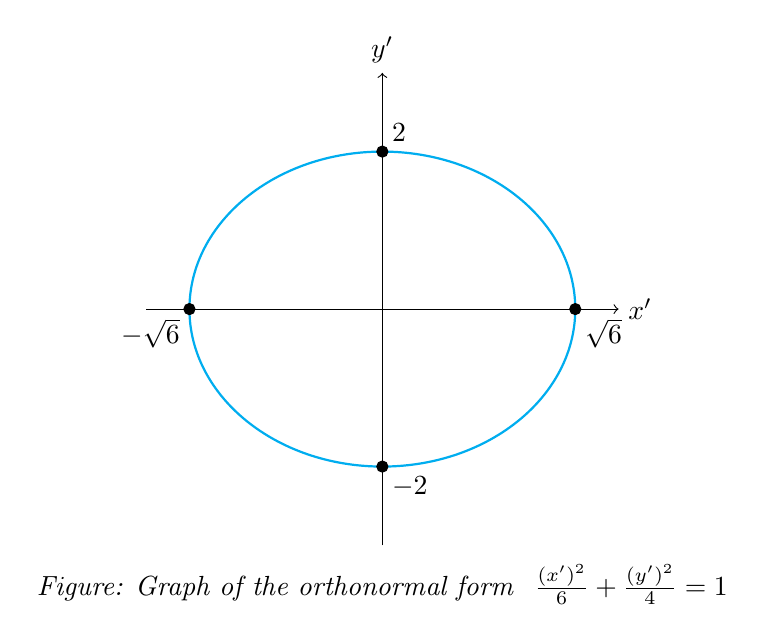
\begin{tikzpicture}
		% Draw Axes
		\draw[->] (-3,0) -- (3,0) node[right] {$x'$};
		\draw[->] (0,-3) -- (0,3) node[above] {$y'$};

		% Draw Ellipse
		\draw[thick, cyan] (0,0) ellipse (2.45cm and 2cm);

		% Label intercepts
		\filldraw (2.45,0) circle (2pt) node[anchor=north west] {$\sqrt{6}$};
		\filldraw (-2.45,0) circle (2pt) node[anchor=north east] {$-\sqrt{6}$};
		\filldraw (0,2) circle (2pt) node[anchor=south west] {$2$};
		\filldraw (0,-2) circle (2pt) node[anchor=north west] {$-2$};

		\node at (0,-3.5) {\textit{Figure: Graph of the orthonormal form } $\frac{(x')^2}{6} + \frac{(y')^2}{4} = 1$};
	\end{tikzpicture}
\end{center}

\pagebreak

% Question 16

\section{Question 16}
\textbf{Problem}
Determine whether the given matrix $A$ is diagonalizable. \\
If so, find the matrix $P$ that diagonalizes $A$ and the diagonal matrix $D$
such that $D = P^{-1}AP$.
\[
	A =
	\begin{bmatrix}
		1            & 2 \\
		-\frac{1}{2} & 1
	\end{bmatrix}
\]
\\
\\
\textbf{Solution}
\textbf{Step 1. Find Eigenvalues}
We find the eigenvalues by solving the characteristic equation
$\det(A - \lambda I) = 0$:
\begin{align*}
	\begin{vmatrix} 1 - \lambda & 2 \\ -1/2 & 1 - \lambda \end{vmatrix} & = 0 \\
	(1 - \lambda)(1 - \lambda) - (2)\left(-\frac{1}{2}\right)           & = 0 \\
	(1 - \lambda)^2 - (-1)                                              & = 0 \\
	(1 - \lambda)^2 + 1                                                 & = 0
\end{align*}
Solving for $\lambda$:
\begin{align*}
	(1 - \lambda)^2 & = -1            \\
	1 - \lambda     & = \pm \sqrt{-1} \\
	1 - \lambda     & = \pm i         \\
	\lambda         & = 1 \pm i
\end{align*}
The eigenvalues are $\lambda_1 = 1 + i$ and $\lambda_2 = 1 - i$.
\\
\\
\textbf{Conclusion}
Since the eigenvalues are complex (not real numbers), there are no corresponding
eigenvectors with real components. Therefore, the matrix $A$ is
\textit{not diagonalizable} over the field of real numbers $\mathbb{R}$.

\pagebreak

% Question 17

\section{Question 17}
\label{sec:q17}
\textbf{Problem}
If $\rho(x,y)$ is the density of a wire (mass per unit length), then
$m = \int_{C}{\rho(x,y)ds}$ is the mass of the wire.
\begin{enumerate}
	\item[i)] Find the mass of a wire having the shape of the semicircle $x=1+\cos t$, $y=\sin t$, $0 \le t \le \pi$, if the density at a point P is directly proportional to its distance from the y-axis.
	\item[ii)] Find the coordinates of the center of mass $(\bar{x}, \bar{y})$.
\end{enumerate}
\textbf{Solution}
\\
\\
\textbf{i) Find the Mass}
The mass is given by the line integral $m = \int_{C}{\rho(x,y)ds}$.
\\
\\
\textbf{1. Parameterization}
\[
	\vec{r}(t) = (1 + \cos{t})\hat{i} + (\sin{t})\hat{j}, \quad 0 \le t \le \pi
\]
\\
\\
\textbf{2. Differential Element $ds$}
Calculate the derivatives:
\[
	\frac{dx}{dt} = -\sin{t}, \quad \frac{dy}{dt} = \cos{t}
\]
Calculate the magnitude:
\[
	ds = \sqrt{\left(-\sin{t}\right)^{2} + \left(\cos{t}\right)^{2}} \, dt = \sqrt{\sin^{2}{t} + \cos^{2}{t}} \, dt = 1 \, dt
\]
\\
\\
\textbf{3. Density Function}
The density is proportional to the distance from the y-axis ($|x|$). Since $x = 1 + \cos{t} \ge 0$ for the given domain:
\[
	\rho(x,y) = kx = k(1 + \cos{t})
\]
where $k$ is a constant of proportionality.
\\
\\
\textbf{4. Integral for Mass}
\begin{align*}
	m & = \int_{0}^{\pi}{k(1 + \cos t)(1)dt}    \\
	  & = k \left[ t + \sin t \right]_{0}^{\pi} \\
	  & = k [(\pi + 0) - (0 + 0)]               \\
	  & = k\pi
\end{align*}
\\
\\
\textbf{ii) Find Center of Mass}
The coordinates are given by $\bar{x} = M_{y}/m$ and
$\bar{y} = M_{x}/m$.
\\
\\
\textbf{Calculate $M_{y}$ (Moment about y-axis):}
\[
	M_{y} = \int_{C}{x \rho(x,y)ds} = \int_{0}^{\pi}{(1 + \cos{t}) k(1 + \cos{t})dt}
\]
\[
	M_{y} = k \int_{0}^{\pi}{(1 + \cos{t})^{2}dt} = k \int_{0}^{\pi}{(1 + 2\cos{t} + \cos^{2}{t})dt}
\]
Using the identity $\cos^{2}{t} = (1 + \cos{2t})/2$ :
\begin{align*}
	M_y & = k \int_{0}^{\pi}{\left( 1 + 2\cos{t} + \frac{1}{2} + \frac{1}{2}\cos{2t} \right)dt} \\
	    & = k \int_{0}^{\pi}{\left( \frac{3}{2} + 2\cos{t} + \frac{1}{2}\cos{2t} \right)dt}     \\
	    & = k \left[\frac{3}{2}t + 2\sin{t} + \frac{1}{4}\sin{2t} \right]_{0}^{\pi}             \\
	    & = k \left[\left(\frac{3\pi}{2} + 0 + 0\right) - 0 \right] = \frac{3\pi k}{2}
\end{align*}
\[
	\bar{x} = \frac{M_y}{m} = \frac{3\pi k / 2}{k\pi} = \frac{3}{2}
\]
\\
\\
\textbf{Calculate $M_{x}$ (Moment about x-axis):}
\[
	M_{x} = \int_{C}{y \rho(x,y)ds} = \int_{0}^{\pi}{(\sin t) k(1 + \cos t)dt}
\]
\[
	M_{x} = k \int_{0}^{\pi}{(\sin t + \sin t \cos t)dt}
\]
Using simple integration for $\sin{t}$ and $u$-substitution (or identity
$\sin{2t}$) for $\sin{t} \cos{t}$:
\begin{align*}
	M_{x} & = k \left[ -\cos{t} + \frac{1}{2}\sin^{2}{t} \right]_{0}^{\pi} \\
	      & = k \left[ (-\cos{\pi} + 0) - (-\cos{0} + 0) \right]           \\
	      & = k \left[ -(-1) - (-1) \right] = k(1 + 1) = 2k
\end{align*}
\[
	\bar{y} = \frac{M_{x}}{m} = \frac{2k}{k\pi} = \frac{2}{\pi}
\]
\\
\\
\textbf{Answer}
The mass is $m = k\pi$, and the center of mass is located at
$\left(3/2, 2/\pi\right)$.

\pagebreak

% Question 18

\section{Question 18}
\textbf{Problem}
If $u = f(x,y)$ and $x = r\cos{\theta}, y = r\sin{\theta}$, show that Laplace's
Equation
\[
	\frac{\partial^{2}u}{\partial r^{2}}+\frac{1}{r}\frac{\partial u}{\partial r}+\frac{1}{r^{2}}\frac{\partial^{2}u}{\partial\theta^{2}}=0
\]
\\
\\
\textbf{Solution}
We perform the change of variables using the Chain Rule.
Given:
\[
	x = r\cos\theta, \quad y = r\sin\theta \implies r = \sqrt{x^2+y^2}, \quad \theta = \arctan\left(\frac{y}{x}\right)
\]
\\
\\
\textbf{Step 1. First Partial Derivatives of Coordinates}
We calculate the derivatives of $r$ and $\theta$ with respect to $x$ and $y$:
\begin{align*}
	\frac{\partial r}{\partial x}      & = \frac{x}{\sqrt{x^2+y^2}} = \frac{r\cos\theta}{r} = \cos\theta                           & \frac{\partial r}{\partial y}      & = \sin\theta           \\
	\frac{\partial \theta}{\partial x} & = \frac{1}{1+(y/x)^2}\left(-\frac{y}{x^2}\right) = -\frac{y}{r^2} = -\frac{\sin\theta}{r} & \frac{\partial \theta}{\partial y} & = \frac{\cos\theta}{r}
\end{align*}
\\
\\
\textbf{Step 2. First Partial Derivative of $u$}
Using the chain rule: $\frac{\partial u}{\partial x} = \frac{\partial u}{\partial r}\frac{\partial r}{\partial x} + \frac{\partial u}{\partial \theta}\frac{\partial \theta}{\partial x}$:
\begin{equation} \label{ux}
	u_x = (\cos\theta)u_r - \left(\frac{\sin\theta}{r}\right)u_\theta
\end{equation}
Similarly for $y$:
\begin{equation} \label{uy}
	u_y = (\sin\theta)u_r + \left(\frac{\cos\theta}{r}\right)u_\theta
\end{equation}
\\
\\
\textbf{Step 3. Second Partial Derivative $u_{xx}$}
We apply the operator $\frac{\partial}{\partial x} = \cos\theta \frac{\partial}{\partial r} - \frac{\sin\theta}{r} \frac{\partial}{\partial \theta}$ to equation (\ref{ux}).
\textit{(Note: We must use the product rule because the coefficients depend on
	$r$ and $\theta$)}
\begin{align*}
	u_{xx} & = \frac{\partial}{\partial x}\left( \cos\theta \cdot u_r - \frac{\sin\theta}{r} \cdot u_\theta \right)                                                                                                                                          \\
	       & = \cos\theta \frac{\partial}{\partial x}(u_r) + u_r \frac{\partial}{\partial x}(\cos\theta) - \left[ \frac{\sin\theta}{r} \frac{\partial}{\partial x}(u_\theta) + u_\theta \frac{\partial}{\partial x}\left(\frac{\sin\theta}{r}\right) \right]
\end{align*}
Expanding terms individually is tedious. A cleaner way is to apply the full operator to the full expression:
\begin{align*}
	u_{xx} & = \left( \cos\theta \partial_r - \frac{\sin\theta}{r} \partial_\theta \right) \left( \cos\theta u_r - \frac{\sin\theta}{r} u_\theta \right)                                           \\
	       & = \cos^2\theta u_{rr} - \frac{2\sin\theta\cos\theta}{r}u_{r\theta} + \frac{\sin^2\theta}{r^2}u_{\theta\theta} + \frac{\sin^2\theta}{r}u_r + \frac{2\sin\theta\cos\theta}{r^2}u_\theta
\end{align*}
\\
\\
\textbf{Step 4. Second Partial Derivative $u_{yy}$}
We apply $\frac{\partial}{\partial y} = \sin\theta \frac{\partial}{\partial r} + \frac{\cos\theta}{r} \frac{\partial}{\partial \theta}$ to equation (\ref{uy}):
\begin{align*}
	u_{yy} & = \left( \sin\theta \partial_r + \frac{\cos\theta}{r} \partial_\theta \right) \left( \sin\theta u_r + \frac{\cos\theta}{r} u_\theta \right)                                           \\
	       & = \sin^2\theta u_{rr} + \frac{2\sin\theta\cos\theta}{r}u_{r\theta} + \frac{\cos^2\theta}{r^2}u_{\theta\theta} + \frac{\cos^2\theta}{r}u_r - \frac{2\sin\theta\cos\theta}{r^2}u_\theta
\end{align*}
\\
\\
\textbf{Step 5. Summation $u_{xx} + u_{yy}$}
Adding the two expanded expressions:
\begin{align*}
	u_{xx} + u_{yy} & = (\cos^2\theta + \sin^2\theta)u_{rr}                                             \\
	                & \quad + \frac{1}{r}(\sin^2\theta + \cos^2\theta)u_r                               \\
	                & \quad + \frac{1}{r^2}(\sin^2\theta + \cos^2\theta)u_{\theta\theta}                \\
	                & \quad + \text{(Terms with } u_{r\theta} \text{ and } u_\theta \text{ cancel out)}
\end{align*}
Since $\cos^2\theta + \sin^2\theta = 1$, we arrive at the final form:
\[
	\nabla^2 u = u_{rr} + \frac{1}{r}u_r + \frac{1}{r^2}u_{\theta\theta} = 0
\]
This completes the derivation.

\pagebreak

% Question 19

\section{Question 19}
\textbf{Problem}
The temperature $T$ at a point $(x,y,z)$ is inversely proportional to the square
of the distance from the origin.
Given $T(0,0,1)=500$:
\begin{enumerate}
	\item Find the rate of change of $T$ at $(2,3,3)$ in the direction of $(3,1,1)$.
	\item In which direction does $T$ increase most rapidly?
	\item What is the maximum rate of change?
\end{enumerate}
\textbf{Solution}
\\
\\
\textbf{Step 1. Define the Temperature Function}
Let $r$ be the distance from the origin, $r^2 = x^2 + y^2 + z^2$.
The problem states $T = \frac{k}{r^2} = \frac{k}{x^2+y^2+z^2}$.
\\
Using the condition $T(0,0,1) = 500$:
\[
	500 = \frac{k}{0^2 + 0^2 + 1^2} \implies k = 500
\]
So, $T(x,y,z) = 500(x^2 + y^2 + z^2)^{-1}$.
\\
\\
\textbf{Step 2. Calculate the Gradient $\nabla T$}
We compute the partial derivatives:
\begin{align*}
	\frac{\partial T}{\partial x} & = -500(x^2+y^2+z^2)^{-2}(2x) = -\frac{1000x}{(x^2+y^2+z^2)^2} \\
	\frac{\partial T}{\partial y} & = -\frac{1000y}{(x^2+y^2+z^2)^2}                              \\
	\frac{\partial T}{\partial z} & = -\frac{1000z}{(x^2+y^2+z^2)^2}
\end{align*}
\[
	\nabla T = -\frac{1000}{(x^2+y^2+z^2)^2} \langle x, y, z \rangle
\]
\\
\\
\textbf{Step 3. Evaluate Gradient at $P(2,3,3)$}
First, calculate the squared distance at $P$:
\[
	r^2 = 2^2 + 3^2 + 3^2 = 4 + 9 + 9 = 22
\]
Now substitute into the gradient expression:
\[
	\nabla T(2,3,3) = -\frac{1000}{(22)^2} \langle 2, 3, 3 \rangle = -\frac{1000}{484} \langle 2, 3, 3 \rangle = -\frac{250}{121} \langle 2, 3, 3 \rangle
\]
\[
	\nabla T = \left\langle -\frac{500}{121}, -\frac{750}{121}, -\frac{750}{121} \right\rangle
\]
\\
\\
\textbf{Part 1. Rate of Change in Direction $\vec{v} = (3,1,1)$}
We need the unit vector $\vec{u}$ in the direction of $\vec{v}$:
\[
	|\vec{v}| = \sqrt{3^2 + 1^2 + 1^2} = \sqrt{9+1+1} = \sqrt{11}
\]
\[
	\vec{u} = \frac{1}{\sqrt{11}}\langle 3, 1, 1 \rangle
\]
The directional derivative is $D_{\vec{u}}T = \nabla T \cdot \vec{u}$:
\begin{align*}
	D_{\vec{u}}T & = \left( -\frac{250}{121} \langle 2, 3, 3 \rangle \right) \cdot \left( \frac{1}{\sqrt{11}} \langle 3, 1, 1 \rangle \right) \\
	             & = -\frac{250}{121\sqrt{11}} \left( (2)(3) + (3)(1) + (3)(1) \right)                                                        \\
	             & = -\frac{250}{121\sqrt{11}} (6 + 3 + 3) = -\frac{250(12)}{121\sqrt{11}}                                                    \\
	             & = -\frac{3000}{121\sqrt{11}} \approx -7.47
\end{align*}
\\
\\
\textbf{Part 2. Direction of Most Rapid Increase}
Temperature increases most rapidly in the direction of the gradient vector $\nabla T$.
\[
	\text{Direction} = \nabla T = -\frac{250}{121} \langle 2, 3, 3 \rangle
\]
Since the scalar is negative, this vector points towards the origin (opposite to the position vector).
Normalized direction: $\vec{u}_{max} = \frac{\langle -2, -3, -3 \rangle}{\sqrt{22}}$.
\\
\\
\textbf{Part 3. Maximum Rate of Change}
The maximum rate is the magnitude of the gradient vector $|\nabla T|$:
\begin{align*}
	|\nabla T| & = \left| -\frac{250}{121} \langle 2, 3, 3 \rangle \right| \\
	           & = \frac{250}{121} \sqrt{2^2 + 3^2 + 3^2}                  \\
	           & = \frac{250}{121} \sqrt{22} \approx 9.69
\end{align*}

\pagebreak

% Question 20 - half way done

\section{Question 20}
\textbf{Problem}
Any scalar function $f$ for which $\nabla^{2}f=0$ (Laplace's Equation) is said
to be harmonic. Verify that $f(x,y,z)=(x^{2}+y^{2}+z^{2})^{-1/2}$ is harmonic
except at the origin.
\\
\\
\textbf{Solution}
Let $r = \sqrt{x^2+y^2+z^2}$. The function can be written as
$f = r^{-1} = (x^2+y^2+z^2)^{-1/2}$.
We need to show that
$\nabla^2 f = \frac{\partial^2 f}{\partial x^2} + \frac{\partial^2 f}{\partial y^2} + \frac{\partial^2 f}{\partial z^2} = 0$.
\\
\\
\textbf{Step 1. Partial Derivatives with respect to $x$}
First derivative:
\begin{align*}
	\frac{\partial f}{\partial x} & = -\frac{1}{2}(x^2+y^2+z^2)^{-3/2} \cdot (2x) \\
	                              & = -x(x^2+y^2+z^2)^{-3/2}
\end{align*}
Second derivative (using Product Rule):
\begin{align*}
	\frac{\partial^2 f}{\partial x^2} & = \frac{\partial}{\partial x} \left[ -x(x^2+y^2+z^2)^{-3/2} \right]                          \\
	                                  & = (-1)(x^2+y^2+z^2)^{-3/2} + (-x) \left[ -\frac{3}{2}(x^2+y^2+z^2)^{-5/2} \cdot (2x) \right] \\
	                                  & = -(x^2+y^2+z^2)^{-3/2} + 3x^2(x^2+y^2+z^2)^{-5/2}
\end{align*}
To combine terms, multiply the first term by $\frac{x^2+y^2+z^2}{x^2+y^2+z^2}$:
\begin{align*}
	\frac{\partial^2 f}{\partial x^2} & = \frac{-(x^2+y^2+z^2) + 3x^2}{(x^2+y^2+z^2)^{5/2}} = \frac{2x^2 - y^2 - z^2}{(x^2+y^2+z^2)^{5/2}}
\end{align*}
\\
\\
\textbf{Step 2. Partial Derivatives with respect to $y$ and $z$}
By symmetry, the derivatives for $y$ and $z$ follow the exact same pattern:
\[
	\frac{\partial^2 f}{\partial y^2} = \frac{2y^2 - x^2 - z^2}{(x^2+y^2+z^2)^{5/2}}
\]
\[
	\frac{\partial^2 f}{\partial z^2} = \frac{2z^2 - x^2 - y^2}{(x^2+y^2+z^2)^{5/2}}
\]
\\
\\
\textbf{Step 3. Summation}
Summing the numerators:
\begin{align*}
	\text{Numerator} & = (2x^2 - y^2 - z^2) + (2y^2 - x^2 - z^2) + (2z^2 - x^2 - y^2) \\
	                 & = (2x^2 - x^2 - x^2) + (2y^2 - y^2 - y^2) + (2z^2 - z^2 - z^2) \\
	                 & = 0 + 0 + 0 = 0
\end{align*}
Thus:
\[
	\nabla^2 f = \frac{0}{(x^2+y^2+z^2)^{5/2}} = 0
\]
Since the Laplacian is zero for all points where $x^2+y^2+z^2 \neq 0$, the
function is harmonic everywhere except at the origin.

\pagebreak

% Question 21

\section{Question 21}
\textbf{Problem}
Evaluate $\oint_C \vec{f} \cdot d\vec{r}$ for the path
$C = C_1 + C_2 + C_3 + C_4$ shown in the figure, where
$\vec{f}(x,y,z) = (y-x^2)\hat{i} + (x-y^2z)\hat{j} - yz^2\hat{k}$. The vertices
are $A(2,1,0)$, $B(0,1,0)$, $C(0,1,2)$, and $D(2,0,0)$.
\\
\\
\textbf{Solution}
\\
\\
\textbf{1. Segment $C_1$: From $D(2,0,0)$ to $B(0,1,0)$}
\\
Parameterization: $x$ goes from 2 to 0, $y$ goes from 0 to 1, $z=0$.
Let $x = 2 - 2t, \quad y = t, \quad z = 0$ for $t \in [0, 1]$.
\\
Differentials: $dx = -2dt, \quad dy = dt, \quad dz = 0$.
Substitute into the integral:
\begin{align*}
	I_1 & = \int_0^1 \left[ (t - (2-2t)^2)(-2) + ((2-2t) - t^2(0))(1) + 0 \right] dt              \\
	    & = \int_0^1 \left[ -2(t - (4 - 8t + 4t^2)) + 2 - 2t \right] dt                           \\
	    & = \int_0^1 \left[ -2t + 8 - 16t + 8t^2 + 2 - 2t \right] dt                              \\
	    & = \int_0^1 \left[ 8t^2 - 20t + 10 \right] dt                                            \\
	    & = \left[ \frac{8}{3}t^3 - 10t^2 + 10t \right]_0^1 = \frac{8}{3} - 10 + 10 = \frac{8}{3}
\end{align*}
\\
\\
\textbf{2. Segment $C_2$: From $B(0,1,0)$ to $C(0,1,2)$}
\\
Parameterization: $x=0, y=1, z=t$ for $t \in [0, 2]$.
\\
Differentials: $dx=0, dy=0, dz=dt$.
\begin{align*}
	I_2 & = \int_0^2 \left[ -yz^2 \right] dt = \int_0^2 -(1)(t^2) dt \\
	    & = \left[ -\frac{t^3}{3} \right]_0^2 = -\frac{8}{3}
\end{align*}
\\
\\
\textbf{3. Segment $C_3$: From $C(0,1,2)$ to $A(2,1,0)$}
\\
Parameterization: $x=2t, y=1, z=2-2t$ for $t \in [0, 1]$.
\\
Differentials: $dx=2dt, dy=0, dz=-2dt$.
\begin{align*}
	I_3 & = \int_0^1 \left[ (1 - (2t)^2)(2) + 0 - (1)(2-2t)^2(-2) \right] dt \\
	    & = \int_0^1 \left[ 2(1 - 4t^2) + 2(2-2t)^2 \right] dt               \\
	    & = \int_0^1 \left[ 2 - 8t^2 + 2(4 - 8t + 4t^2) \right] dt           \\
	    & = \int_0^1 \left[ 2 - 8t^2 + 8 - 16t + 8t^2 \right] dt             \\
	    & = \int_0^1 (10 - 16t) dt                                           \\
	    & = \left[ 10t - 8t^2 \right]_0^1 = 10 - 8 = 2
\end{align*}
\\
\\
\textbf{4. Segment $C_4$: From $A(2,1,0)$ to $D(2,0,0)$}
\\
Parameterization: $x=2, z=0, y$ goes from 1 to 0.
Let $y = t$ from 1 to 0.
\\
Differentials: $dx=0, dz=0, dy=dt$.
\begin{align*}
	I_4 & = \int_1^0 \left[ (x - y^2z) \right] dy = \int_1^0 (2 - y^2(0)) dy \\
	    & = \int_1^0 2 dy = [2y]_1^0 = 0 - 2 = -2
\end{align*}
\\
\\
\textbf{Total Integral}
\[
	\oint_C \vec{f} \cdot d\vec{r} = I_1 + I_2 + I_3 + I_4 = \frac{8}{3} - \frac{8}{3} + 2 - 2 = 0
\]
\textbf{Final Answer } The value of the line integral is 0.

\pagebreak

% Question 22

\section{Question 22}
\textbf{Problem}
If $\vec{f} = (2xy - x^2)\hat{i} + (x + y^2)\hat{j}$, verify Green's Theorem in
the plane where $S$ is the closed region bounded by $y=x^2$ and $x=y^2$. The
path $C = C_1 + C_2$ is shown in the figure.
\\
\\
\textbf{Solution}
Green's Theorem states:
\[
	\oint_C \vec{f} \cdot d\vec{r} = \iint_S \left( \frac{\partial M}{\partial x} - \frac{\partial L}{\partial y} \right) dA
\]
where $\vec{f} = L\hat{i} + M\hat{j}$.
\\
Given: $L = 2xy - x^2$ and $M = x + y^2$.
\\
\\
\textbf{Part 1. The Double Integral}
We compute the partial derivatives:
\[
	\frac{\partial M}{\partial x} = 1, \quad \frac{\partial L}{\partial y} = 2x
\]
\[
	\text{Integrand} = \frac{\partial M}{\partial x} - \frac{\partial L}{\partial y} = 1 - 2x
\]
The region $S$ is bounded by $y=x^2$ (lower curve) and $y=\sqrt{x}$ (upper curve) from $x=0$ to $x=1$.
\begin{align*}
	\iint_S (1 - 2x) \, dy \, dx & = \int_0^1 \int_{x^2}^{\sqrt{x}} (1 - 2x) \, dy \, dx                                                       \\
	                             & = \int_0^1 (1 - 2x) [y]_{x^2}^{\sqrt{x}} \, dx                                                              \\
	                             & = \int_0^1 (1 - 2x)(\sqrt{x} - x^2) \, dx                                                                   \\
	                             & = \int_0^1 (x^{1/2} - x^2 - 2x^{3/2} + 2x^3) \, dx                                                          \\
	                             & = \left[ \frac{2}{3}x^{3/2} - \frac{x^3}{3} - 2\left(\frac{2}{5}x^{5/2}\right) + \frac{2x^4}{4} \right]_0^1 \\
	                             & = \left( \frac{2}{3} - \frac{1}{3} - \frac{4}{5} + \frac{1}{2} \right) - 0                                  \\
	                             & = \frac{1}{3} - \frac{4}{5} + \frac{1}{2}                                                                   \\
	                             & = \frac{10}{30} - \frac{24}{30} + \frac{15}{30}                                                             \\
	                             & = \frac{1}{30}
\end{align*}
\\
\\
\textbf{Part 2. The Line Integral}
The line integral is $\oint_C (2xy - x^2)dx + (x + y^2)dy$.
\\
\\
\textbf{Segment $C_1$: Along $y=x^2$ from $(0,0)$ to $(1,1)$}
Let $x=t, y=t^2$ for $t \in [0, 1]$. Then $dx=dt, dy=2t dt$.
\begin{align*}
	I_1 & = \int_0^1 \left[ (2(t)(t^2) - t^2)(1) + (t + (t^2)^2)(2t) \right] dt               \\
	    & = \int_0^1 \left[ (2t^3 - t^2) + (2t^2 + 2t^5) \right] dt                           \\
	    & = \int_0^1 (2t^5 + 2t^3 + t^2) dt                                                   \\
	    & = \left[ \frac{2t^6}{6} + \frac{2t^4}{4} + \frac{t^3}{3} \right]_0^1                \\
	    & = \frac{1}{3} + \frac{1}{2} + \frac{1}{3} = \frac{2}{3} + \frac{1}{2} = \frac{7}{6}
\end{align*}
\\
\\
\textbf{Segment $C_2$: Along $x=y^2$ from $(1,1)$ to $(0,0)$}
Let $y=t$ from $t=1$ to $0$. Then $x=t^2, dx=2t dt$.
\begin{align*}
	I_2 & = \int_1^0 \left[ (2(t^2)(t) - (t^2)^2)(2t) + (t^2 + t^2)(1) \right] dt                                       \\
	    & = \int_1^0 \left[ (2t^3 - t^4)(2t) + 2t^2 \right] dt                                                          \\
	    & = \int_1^0 (4t^4 - 2t^5 + 2t^2) dt                                                                            \\
	    & = \left[ \frac{4t^5}{5} - \frac{2t^6}{6} + \frac{2t^3}{3} \right]_1^0                                         \\
	    & = 0 - \left( \frac{4}{5} - \frac{1}{3} + \frac{2}{3} \right)                                                  \\
	    & = - \left( \frac{4}{5} + \frac{1}{3} \right) = - \left( \frac{12}{15} + \frac{5}{15} \right) = -\frac{17}{15}
\end{align*}
\\
\\
\textbf{Total Line Integral}
\[
	\oint_C \vec{f} \cdot d\vec{r} = I_1 + I_2 = \frac{7}{6} - \frac{17}{15}
\]
Find common denominator (30):
\[
	\frac{35}{30} - \frac{34}{30} = \frac{1}{30}
\]
\textbf{Conclusion}
Since the double integral $\left(\frac{1}{30}\right)$ equals the line integral
$\left(\frac{1}{30}\right)$, Green's Theorem is verified.

\pagebreak

% Question 23

\section{Question 23}
\textbf{Problem}
Verify Stokes' Theorem
$\iint_S (\nabla \times \vec{f}) \cdot d\vec{s} = \oint_C \vec{f} \cdot d\vec{r}$
for the vector field $\vec{f} = xz^2\hat{i} - yx\hat{j} + zy^2\hat{k}$, where $S$
is the upper hemisphere $x^2 + y^2 + z^2 = 9$ ($0 \le z \le 3$) and $C$ is its
circular boundary on the $xy$-plane.
\\
\\
\textbf{Solution}
\\
\\
\textbf{Part 1. The Line Integral}
The boundary $C$ is the circle $x^2 + y^2 = 9$ on the plane $z=0$.
Since $z=0$ everywhere on $C$, we have $dz=0$.
Substituting $z=0$ into the vector field $\vec{f}$:
\[
	\vec{f}(x,y,0) = x(0)^2\hat{i} - yx\hat{j} + (0)y^2\hat{k} = -yx\hat{j}
\]
The line integral simplifies to:
\[
	\oint_C \vec{f} \cdot d\vec{r} = \oint_C (0 dx - yx dy + 0 dz) = \oint_C -xy \, dy
\]
We parameterize the circle $C$ (counter-clockwise, radius 3):
\[
	x = 3\cos t, \quad y = 3\sin t, \quad dy = 3\cos t \, dt, \quad t \in [0, 2\pi]
\]
Substitute into the integral:
\begin{align*}
	I & = \int_0^{2\pi} -(3\cos t)(3\sin t)(3\cos t) \, dt \\
	  & = -27 \int_0^{2\pi} \cos^2 t \sin t \, dt
\end{align*}
Let $u = \cos t$, then $du = -\sin t \, dt$.
Limits: $t=0 \implies u=1$, $t=2\pi \implies u=1$.
\[
	I = -27 \int_1^1 u^2 (-du) = 0
\]
\textbf{Result} The line integral is \textbf{0}.
\\
\\
\textbf{Part 2. The Surface Integral}
First, we compute the Curl of $\vec{f}$:
\[
	\nabla \times \vec{f} = \begin{vmatrix} \hat{i} & \hat{j} & \hat{k} \\ \partial_x & \partial_y & \partial_z \\ xz^2 & -yx & zy^2 \end{vmatrix}
\]
\begin{align*}
	\text{$\hat{i}$-component:} & \quad \frac{\partial}{\partial y}(zy^2) - \frac{\partial}{\partial z}(-yx) = 2zy - 0 = 2yz                     \\
	\text{$\hat{j}$-component:} & \quad -\left( \frac{\partial}{\partial x}(zy^2) - \frac{\partial}{\partial z}(xz^2) \right) = -(0 - 2xz) = 2xz \\
	\text{$\hat{k}$-component:} & \quad \frac{\partial}{\partial x}(-yx) - \frac{\partial}{\partial y}(xz^2) = -y - 0 = -y
\end{align*}
\[
	\nabla \times \vec{f} = \langle 2yz, 2xz, -y \rangle
\]
The outward unit normal for the sphere $x^2+y^2+z^2=9$ is $\hat{n} = \frac{1}{3}\langle x, y, z \rangle$.
We calculate the dot product $(\nabla \times \vec{f}) \cdot \hat{n}$:
\begin{align*}
	(\nabla \times \vec{f}) \cdot \hat{n} & = \frac{1}{3} \left[ (2yz)(x) + (2xz)(y) + (-y)(z) \right] \\
	                                      & = \frac{1}{3} [ 2xyz + 2xyz - yz ]                         \\
	                                      & = \frac{1}{3} [ 4xyz - yz ]
\end{align*}
We now integrate this scalar field over the hemisphere using spherical coordinates:
\[
	x = 3\sin\phi\cos\theta, \quad y = 3\sin\phi\sin\theta, \quad z = 3\cos\phi
\]
The area element is $dS = 9 \sin\phi \, d\phi \, d\theta$.
The integral splits into two terms:
\[
	I_S = \iint_S \frac{4}{3}xyz \, dS - \iint_S \frac{1}{3}yz \, dS
\]
\\
\\
\textbf{Term 1 analysis ($4xyz$):}
The term involves the product
$xy \propto \cos\theta \sin\theta = \frac{1}{2}\sin(2\theta)$. Integration with
respect to $\theta$ from $0$ to $2\pi$:
\[
	\int_0^{2\pi} \sin(2\theta) \, d\theta = 0 \implies \text{The first term vanishes.}
\]
\\
\\
\textbf{Term 2 analysis ($-yz$):}
The term involves $y \propto \sin\theta$.
Integration with respect to $\theta$ from $0$ to $2\pi$:
\[
	\int_0^{2\pi} \sin\theta \, d\theta = 0 \implies \text{The second term vanishes.}
\]
\\
\\
\textbf{Conclusion}
\\
Since both terms integrate to zero due to symmetry:
\[
	\iint_S (\nabla \times \vec{f}) \cdot d\vec{s} = 0
\]
Both the line integral and surface integral yield 0, verifying Stokes' Theorem.

\pagebreak

% Question 24

\section{Question 24}
\textbf{Problem}
Verify Stokes' Theorem
$\iint_S (\nabla \times \vec{f}) \cdot d\vec{s} = \oint_C \vec{f} \cdot d\vec{r}$
for the vector field $\vec{f} = y\hat{i} + z\hat{j} + x\hat{k}$. The surface $S$
is the paraboloid $z = 1 - (x^2 + y^2)$ for $z \ge 0$, bounded by the circle $C$
in the $xy$-plane.
\\
\\
\textbf{Solution}
\\
\\
\textbf{Part 1. The Line Integral}
The boundary curve $C$ is the circle $x^2 + y^2 = 1$ lying in the plane $z=0$.
Orientation is counter-clockwise (standard positive orientation).
\\
\\
\textbf{Parameterization}
Let $x = \cos t$, $y = \sin t$, $z = 0$ for $t \in [0, 2\pi]$.
The differential vector $d\vec{r}$ is:
\[
	d\vec{r} = \langle -\sin t, \cos t, 0 \rangle \, dt
\]
Substitute the coordinates into the vector field $\vec{f} = \langle y, z, x \rangle$:
\[
	\vec{f}(t) = \langle \sin t, 0, \cos t \rangle
\]
\textit{(Note: $y=\sin t$, $z=0$, $x=\cos t$)}
\\
\\
\textbf{Calculate Dot Product}
\begin{align*}
	\vec{f} \cdot d\vec{r} & = \langle \sin t, 0, \cos t \rangle \cdot \langle -\sin t, \cos t, 0 \rangle \\
	                       & = (\sin t)(-\sin t) + (0)(\cos t) + (\cos t)(0)                              \\
	                       & = -\sin^2 t
\end{align*}
\\
\\
\textbf{Evaluate Integral}
\begin{align*}
	\oint_C \vec{f} \cdot d\vec{r} & = \int_0^{2\pi} -\sin^2 t \, dt                               \\
	                               & = -\int_0^{2\pi} \frac{1 - \cos(2t)}{2} \, dt                 \\
	                               & = -\frac{1}{2} \left[ t - \frac{\sin(2t)}{2} \right]_0^{2\pi} \\
	                               & = -\frac{1}{2} [ (2\pi - 0) - (0 - 0) ]                       \\
	                               & = -\pi
\end{align*}
\\
\\
\textbf{Part 2. The Surface Integral}
First, calculate the Curl of $\vec{f} = \langle y, z, x \rangle$:
\[
	\nabla \times \vec{f} = \begin{vmatrix} \hat{i} & \hat{j} & \hat{k} \\ \partial_x & \partial_y & \partial_z \\ y & z & x \end{vmatrix}
\]
\begin{align*}
	\text{$\hat{i}$-component:} & \quad \frac{\partial}{\partial y}(x) - \frac{\partial}{\partial z}(z) = 0 - 1 = -1 \\
	\text{$\hat{j}$-component:} & \quad \frac{\partial}{\partial z}(y) - \frac{\partial}{\partial x}(x) = 0 - 1 = -1 \\
	\text{$\hat{k}$-component:} & \quad \frac{\partial}{\partial x}(z) - \frac{\partial}{\partial y}(y) = 0 - 1 = -1
\end{align*}
\[
	\nabla \times \vec{f} = \langle -1, -1, -1 \rangle
\]
\\
\\
\textbf{Surface Parameterization}
The surface is given explicitly by $z = g(x,y) = 1 - x^2 - y^2$.
For a graph $z=g(x,y)$ with upward orientation, the normal vector $d\vec{s}$ is
given by:
\[
	d\vec{s} = \langle -g_x, -g_y, 1 \rangle \, dA
\]
Calculating partial derivatives of $z$:
\[
	g_x = -2x \implies -g_x = 2x
\]
\[
	g_y = -2y \implies -g_y = 2y
\]
\[
	d\vec{s} = \langle 2x, 2y, 1 \rangle \, dA
\]
\\
\\
\textbf{Calculate Flux Integrand}
\[
	(\nabla \times \vec{f}) \cdot d\vec{s} = \langle -1, -1, -1 \rangle \cdot \langle 2x, 2y, 1 \rangle = -2x - 2y - 1
\]
\\
\\
\textbf{Evaluate Surface Integral}
The domain $D$ is the projection of the paraboloid onto the $xy$-plane, which is
the unit disk $x^2 + y^2 \le 1$. Using polar coordinates:
$x = r\cos\theta, y = r\sin\theta, dA = r \, dr \, d\theta$.
\begin{align*}
	\iint_S (\nabla \times \vec{f}) \cdot d\vec{s} & = \iint_D (-2x - 2y - 1) \, dA                                                    \\
	                                               & = \int_0^{2\pi} \int_0^1 (-2r\cos\theta - 2r\sin\theta - 1) \, r \, dr \, d\theta \\
	                                               & = \int_0^{2\pi} \int_0^1 (-2r^2\cos\theta - 2r^2\sin\theta - r) \, dr \, d\theta
\end{align*}
We can split this into three terms.
\begin{enumerate}
	\item $\int_0^{2\pi} \cos\theta \, d\theta = 0 \implies$ The $x$ term vanishes.
	\item $\int_0^{2\pi} \sin\theta \, d\theta = 0 \implies$ The $y$ term vanishes.
	\item The remaining term is the constant $-1$:
\end{enumerate}
\begin{align*}
	I & = \int_0^{2\pi} d\theta \int_0^1 -r \, dr  \\
	  & = (2\pi) \left[ -\frac{r^2}{2} \right]_0^1 \\
	  & = 2\pi \left( -\frac{1}{2} \right) = -\pi
\end{align*}
\\
\\
\textbf{Conclusion}
\\
Since $\oint_C \vec{f} \cdot d\vec{r} = -\pi$ and
$\iint_S (\nabla \times \vec{f}) \cdot d\vec{s} = -\pi$, Stokes' Theorem is
verified.

\pagebreak

% Question 25

\section{Question 25}
\textbf{Problem}
Verify the Divergence Theorem of Gauss
$\iiint_V (\nabla \cdot \vec{f}) dV = \oiint_S \vec{f} \cdot d\vec{s}$ for the
vector field $\vec{f} = 2x^2y\hat{i} - y^2\hat{j} + 4xz^2\hat{k}$. The volume
$V$ is bounded by $x=0, x=2, y=0, z=0$ and the cylinder $y^2+z^2=9$.
\\
\\
\textbf{Solution}
\\
\\
\textbf{Part 1. The Volume Integral}
First, calculate the divergence of $\vec{f}$:
\begin{align*}
	\nabla \cdot \vec{f} & = \frac{\partial}{\partial x}(2x^2y) + \frac{\partial}{\partial y}(-y^2) + \frac{\partial}{\partial z}(4xz^2) \\
	                     & = 4xy - 2y + 8xz
\end{align*}
We integrate this over the volume $V$. The region is a quarter-cylinder along
the x-axis. It is best described using polar coordinates for $y$ and $z$:
\[
	y = r\cos\theta, \quad z = r\sin\theta, \quad x = x
\]
\\
Limits: $0 \le x \le 2$, $0 \le r \le 3$, $0 \le \theta \le \pi/2$ (First quadrant).
\\
The volume element is $dV = r \, dr \, d\theta \, dx$.
\\
Substituting variables into the divergence:
\[
	\nabla \cdot \vec{f} = 4x(r\cos\theta) - 2(r\cos\theta) + 8x(r\sin\theta)
\]
The integral is:
\[
	I_V = \int_0^{\pi/2} \int_0^3 \int_0^2 (4xr\cos\theta - 2r\cos\theta + 8xr\sin\theta) \, r \, dx \, dr \, d\theta
\]
Integrating with respect to $x$ first ($0$ to $2$):
\begin{align*}
	\int_0^2 (\dots) dx & = \left[ 2x^2 r \cos\theta - 2xr \cos\theta + 4x^2 r \sin\theta \right]_0^2 \\
	                    & = (8r\cos\theta - 4r\cos\theta + 16r\sin\theta) - 0                         \\
	                    & = 4r\cos\theta + 16r\sin\theta
\end{align*}
Now integrate with respect to $r$ ($0$ to $3$), remembering the extra $r$ from
$dV$:
\begin{align*}
	I_V & = \int_0^{\pi/2} \int_0^3 (4r\cos\theta + 16r\sin\theta) r \, dr \, d\theta            \\
	    & = \int_0^{\pi/2} (4\cos\theta + 16\sin\theta) d\theta \int_0^3 r^2 \, dr               \\
	    & = \int_0^{\pi/2} (4\cos\theta + 16\sin\theta) d\theta \left[ \frac{r^3}{3} \right]_0^3 \\
	    & = 9 \int_0^{\pi/2} (4\cos\theta + 16\sin\theta) d\theta
\end{align*}
Finally, integrate with respect to $\theta$:
\begin{align*}
	I_V & = 9 \left[ 4\sin\theta - 16\cos\theta \right]_0^{\pi/2} \\
	    & = 9 [ (4(1) - 0) - (0 - 16(1)) ]                        \\
	    & = 9 [ 4 + 16 ] = 9(20) = 180
\end{align*}
\textit{Volume Integral Result:} $180$.
\\
\\
\textbf{Part 2. The Surface Integral}
We compute the flux through the 5 boundary surfaces.
\\
\\
\textbf{1. Surface $S_1$: $x=0$}
\\
Normal $\hat{n} = -\hat{i}$.
$\vec{f}(0,y,z) = 0\hat{i} - y^2\hat{j} + 0\hat{k}$.
\\
Flux: $\vec{f} \cdot \hat{n} = 0$.
\[ \Phi_1 = 0 \]
\\
\\
\textbf{2. Surface $S_2$: $x=2$}
\\
Normal $\hat{n} = \hat{i}$.
$\vec{f}(2,y,z) = 8y\hat{i} - y^2\hat{j} + 8z^2\hat{k}$.
\\
Flux integrand: $\vec{f} \cdot \hat{i} = 8y$.
\\
Region is the quarter circle ($r=3$) in $yz$-plane.
\begin{align*}
	\Phi_2 = \int_0^{\pi/2} \int_0^3 (8r\cos\theta) r \, dr \, d\theta & = 8 \left(\int \cos\theta d\theta\right) \left(\int r^2 dr\right)        \\
	                                                                   & = 8 [\sin\theta]_0^{\pi/2} \left[\frac{r^3}{3}\right]_0^3 = 8(1)(9) = 72
\end{align*}
\\
\\
\textbf{3. Surface $S_3$: $y=0$}
\\
Normal $\hat{n} = -\hat{j}$.
$\vec{f}(x,0,z) = 0\hat{i} - 0\hat{j} + 4xz^2\hat{k}$.
\\
Flux integrand: $\vec{f} \cdot (-\hat{j}) = -(-0) = 0$.
\[ \Phi_3 = 0 \]
\\
\\
\textbf{4. Surface $S_4$: $z=0$}
\\
Normal $\hat{n} = -\hat{k}$.
$\vec{f}(x,y,0) = 2x^2y\hat{i} - y^2\hat{j} + 0\hat{k}$.
\\
Flux integrand: $\vec{f} \cdot (-\hat{k}) = 0$.
\[ \Phi_4 = 0 \]
\\
\\
\textbf{5. Surface $S_5$: $y^2+z^2=9$}
The normal vector to the cylinder is in the $yz$-plane.
\\
Gradient $\nabla(y^2+z^2) = 2y\hat{j} + 2z\hat{k}$.
\\
Unit Normal $\hat{n} = \frac{y}{3}\hat{j} + \frac{z}{3}\hat{k}$ (since radius is 3).
\\
Flux integrand:
\begin{align*}
	\vec{f} \cdot \hat{n} & = (2x^2y\hat{i} - y^2\hat{j} + 4xz^2\hat{k}) \cdot \left( 0\hat{i} + \frac{y}{3}\hat{j} + \frac{z}{3}\hat{k} \right) \\
	                      & = -\frac{y^3}{3} + \frac{4xz^3}{3}
\end{align*}
We integrate this over the surface. $dS = R \, d\theta \, dx = 3 \, d\theta \, dx$.
Substitute $y=3\cos\theta, z=3\sin\theta$:
\begin{align*}
	\text{Integrand} & = -\frac{(3\cos\theta)^3}{3} + \frac{4x(3\sin\theta)^3}{3} \\
	                 & = -9\cos^3\theta + 36x\sin^3\theta
\end{align*}
Now integrate over $x \in [0,2]$ and $\theta \in [0, \pi/2]$:
\[
	\Phi_5 = \int_0^2 \int_0^{\pi/2} (-9\cos^3\theta + 36x\sin^3\theta) (3 \, d\theta \, dx)
\]
\[
	\Phi_5 = 3 \left[ \int_0^2 dx \int_0^{\pi/2} -9\cos^3\theta d\theta + \int_0^2 36x dx \int_0^{\pi/2} \sin^3\theta d\theta \right]
\]
Using $\int_0^{\pi/2} \cos^3\theta d\theta = \frac{2}{3}$ and $\int_0^{\pi/2} \sin^3\theta d\theta = \frac{2}{3}$:
\begin{align*}
	\text{Term 1} & = 3(2)(-9)\left(\frac{2}{3}\right) = -36                                                           \\
	\text{Term 2} & = 3\left[\frac{36x^2}{2}\right]_0^2 \left(\frac{2}{3}\right) = 3(72)\left(\frac{2}{3}\right) = 144
\end{align*}
\[
	\Phi_5 = 144 - 36 = 108
\]
\\
\\
\textbf{Total Flux}
\begin{align*}
	\Phi_{total} & = \Phi_1 + \Phi_2 + \Phi_3 + \Phi_4 + \Phi_5 \\
	             & = 0 + 72 + 0 + 0 + 108                       \\
	             & = 180
\end{align*}
\\
\textbf{Conclusion}
\\
Since the Volume Integral ($180$) equals the Surface Integral ($180$), the
Divergence Theorem is verified.

\pagebreak

% Question 26

\section{Question 26}
\textbf{Problem}
Find the shaded area shown in the figure by Green's Theorem in the $xy$-plane:
\[
	\text{Area} = \frac{1}{2} \oint_C (x dy - y dx)
\]
The region is bounded by $y=0$, $y=2-x^2$, and $y=x$. The intersection of $y=x$
and $y=2-x^2$ is at $(1,1)$. The parabola intersects the x-axis at
$(\sqrt{2}, 0)$.
\\
\\
\textbf{Solution}
To find the area using Green's Theorem, we use the vector field
$\vec{F} = (-y/2, x/2)$ or simply the formula:
\[
	A = \frac{1}{2} \oint_C (x \, dy - y \, dx)
\]
We break the path $C$ into three segments $C_1 + C_2 + C_3$.
\\
\\
\textbf{1. Segment $C_1$: Along the x-axis}
\\
Path: From $(0,0)$ to $(\sqrt{2}, 0)$.
\\
Equation: $y=0 \implies dy=0$.
\\
Integral:
\[
	I_1 = \frac{1}{2} \int_0^{\sqrt{2}} (x(0) - (0)dx) = 0
\]
\\
\\
\textbf{2. Segment $C_2$: Along the parabola}
\\
Path: From $(\sqrt{2}, 0)$ to $A(1,1)$.
\\
Equation: $y = 2 - x^2$.
\\
Differentials: $dy = -2x \, dx$.
\\
Substitute into the integral formula:
\begin{align*}
	x \, dy - y \, dx & = x(-2x \, dx) - (2 - x^2) \, dx \\
	                  & = (-2x^2 - 2 + x^2) \, dx        \\
	                  & = (-x^2 - 2) \, dx
\end{align*}
Integrate from $x=\sqrt{2}$ to $x=1$:
\begin{align*}
	I_2 & = \frac{1}{2} \int_{\sqrt{2}}^1 (-x^2 - 2) \, dx                                                           \\
	    & = \frac{1}{2} \left[ -\frac{x^3}{3} - 2x \right]_{\sqrt{2}}^1                                              \\
	    & = \frac{1}{2} \left( \left(-\frac{1}{3} - 2\right) - \left(-\frac{2\sqrt{2}}{3} - 2\sqrt{2}\right) \right) \\
	    & = \frac{1}{2} \left( -\frac{7}{3} - \left( -\frac{8\sqrt{2}}{3} \right) \right)                            \\
	    & = \frac{1}{2} \left( \frac{8\sqrt{2} - 7}{3} \right) = \frac{8\sqrt{2} - 7}{6}
\end{align*}
\\
\\
\textbf{3. Segment $C_3$: Along the line $y=x$}
\\
Path: From $A(1,1)$ to $(0,0)$.
\\
Equation: $y = x \implies dy = dx$.
\\
Substitute into the integral:
\begin{align*}
	x \, dy - y \, dx & = x(dx) - x(dx) = 0
\end{align*}
\[
	I_3 = 0
\]
\\
\\
\textbf{Total Area}
Summing the integrals:
\[
	\text{Area} = I_1 + I_2 + I_3 = 0 + \frac{8\sqrt{2} - 7}{6} + 0
\]
\[
	\text{Area} = \frac{8\sqrt{2} - 7}{6} \approx 0.719
\]
\\
\\
\textbf{Verification (Standard Integration)}
\begin{align*}
	A & = \int_0^1 (x - 0) dx + \int_1^{\sqrt{2}} (2-x^2) dx                            \\
	  & = \left[\frac{x^2}{2}\right]_0^1 + \left[2x - \frac{x^3}{3}\right]_1^{\sqrt{2}} \\
	  & = \frac{1}{2} + \left( \frac{4\sqrt{2}}{3} - \frac{5}{3} \right)                \\
	  & = \frac{3}{6} + \frac{8\sqrt{2} - 10}{6} = \frac{8\sqrt{2} - 7}{6}
\end{align*}
The result is correct.

\pagebreak

% Question 27

\section{Question 27}
\textbf{Problem} \\
i) Find the angle between surfaces $x^2 + y^2 + z^2 = 9$ and $z = x^2 + y^2 - 3$ at the point $P(2, -1, 2)$. \\
ii) Test if any of these scalar functions is a harmonic function. Why?
\\
\\
\textbf{Solution}
\\
\\
\textbf{i) Angle Between the Surfaces}
The angle $\theta$ between two surfaces is defined as the angle between their
normal vectors at the point of intersection. The normal vector to a surface
defined by $f(x,y,z) = c$ is the gradient $\nabla f$.
\\
Let the scalar functions defining the surfaces be:
\[ f(x,y,z) = x^2 + y^2 + z^2 - 9 \]
\[ g(x,y,z) = x^2 + y^2 - z - 3 \]
\\
\\
\textbf{1. Compute Gradients}
\[
	\nabla f = \frac{\partial f}{\partial x}\hat{i} + \frac{\partial f}{\partial y}\hat{j} + \frac{\partial f}{\partial z}\hat{k} = 2x\hat{i} + 2y\hat{j} + 2z\hat{k}
\]
\[
	\nabla g = \frac{\partial g}{\partial x}\hat{i} + \frac{\partial g}{\partial y}\hat{j} + \frac{\partial g}{\partial z}\hat{k} = 2x\hat{i} + 2y\hat{j} - 1\hat{k}
\]
\\
\\
\textbf{2. Evaluate at Point $P(2, -1, 2)$}
Substitute $x=2, y=-1, z=2$:
\[
	\vec{n}_1 = \nabla f(2, -1, 2) = 2(2)\hat{i} + 2(-1)\hat{j} + 2(2)\hat{k} = \langle 4, -2, 4 \rangle
\]
\[
	\vec{n}_2 = \nabla g(2, -1, 2) = 2(2)\hat{i} + 2(-1)\hat{j} - 1\hat{k} = \langle 4, -2, -1 \rangle
\]
\\
\\
\textbf{3. Calculate the Angle}
The cosine of the angle is given by:
\[
	\cos \theta = \frac{|\vec{n}_1 \cdot \vec{n}_2|}{|\vec{n}_1| |\vec{n}_2|}
\]
Dot Product:
\[
	\vec{n}_1 \cdot \vec{n}_2 = (4)(4) + (-2)(-2) + (4)(-1) = 16 + 4 - 4 = 16
\]
Magnitudes:
\[
	|\vec{n}_1| = \sqrt{4^2 + (-2)^2 + 4^2} = \sqrt{16 + 4 + 16} = \sqrt{36} = 6
\]
\[
	|\vec{n}_2| = \sqrt{4^2 + (-2)^2 + (-1)^2} = \sqrt{16 + 4 + 1} = \sqrt{21}
\]
Substitute into the formula:
\[
	\cos \theta = \frac{16}{6\sqrt{21}} = \frac{8}{3\sqrt{21}}
\]
\[
	\theta = \arccos\left( \frac{8}{3\sqrt{21}} \right) \approx \arccos(0.5819) \approx 54.41^\circ
\]
\\
\\
\textbf{ii) Harmonic Function Test}
A function $\phi$ is harmonic if it satisfies Laplace's Equation:
$\nabla^2 \phi = \frac{\partial^2 \phi}{\partial x^2} + \frac{\partial^2 \phi}{\partial y^2} + \frac{\partial^2 \phi}{\partial z^2} = 0$.
\\
\\
\textbf{Test for $f(x,y,z) = x^2 + y^2 + z^2 - 9$:}
\[
	\frac{\partial^2 f}{\partial x^2} = 2, \quad \frac{\partial^2 f}{\partial y^2} = 2, \quad \frac{\partial^2 f}{\partial z^2} = 2
\]
\[
	\nabla^2 f = 2 + 2 + 2 = 6 \neq 0
\]
So, $f$ is \textbf{not} harmonic.
\\
\\
\textbf{Test for $g(x,y,z) = x^2 + y^2 - z - 3$:}
\[
	\frac{\partial^2 g}{\partial x^2} = 2, \quad \frac{\partial^2 g}{\partial y^2} = 2, \quad \frac{\partial^2 g}{\partial z^2} = 0
\]
\[
	\nabla^2 g = 2 + 2 + 0 = 4 \neq 0
\]
So, $g$ is \textbf{not} harmonic.
\\
\\
\textbf{Conclusion}
Neither of the scalar functions defining the surfaces is harmonic because their
Laplacians are non-zero constants.

\pagebreak

% Question 28

\section{Question 28}
\textbf{Problem}
Verify the Divergence Theorem of Gauss (DTG):
$\iiint_V (\nabla \cdot \vec{f}) dV = \oiint_S \vec{f} \cdot d\vec{s}$ for the
vector field:
\[
	\vec{f} = (x^2)\hat{i} + (xz^3(y+1))\hat{j}
\]
The volume $V$ is the pentahedron shown in the figure, bounded by
$x=0, x=2, y=0, z=0$ and the plane $y+z=1$.
\\
\\
\textbf{Solution}
\\
\\
\textbf{Part 1. The Volume Integral}
First, calculate the divergence $\nabla \cdot \vec{f}$:
\[
	\nabla \cdot \vec{f} = \frac{\partial}{\partial x}(x^2) + \frac{\partial}{\partial y}(x(y+1)z^3) + \frac{\partial}{\partial z}(0)
\]
\[
	= 2x + x(1)z^3 + 0 = 2x + xz^3
\]
The volume $V$ is defined by the limits:
$0 \le x \le 2$, $0 \le y \le 1$, and $0 \le z \le 1-y$.
\begin{align*}
	I_V & = \int_0^2 \int_0^1 \int_0^{1-y} (2x + xz^3) \, dz \, dy \, dx                           \\
	    & = \int_0^2 x \, dx \int_0^1 \left[ 2z + \frac{z^4}{4} \right]_0^{1-y} dy                 \\
	    & = \left[ \frac{x^2}{2} \right]_0^2 \int_0^1 \left( 2(1-y) + \frac{(1-y)^4}{4} \right) dy \\
	    & = (2) \int_0^1 \left( 2(1-y) + \frac{1}{4}(1-y)^4 \right) dy
\end{align*}
Let $u = 1-y$, then $du = -dy$. Limits change from $1 \to 0$.
\begin{align*}
	I_V & = 2 \int_1^0 \left( 2u + \frac{u^4}{4} \right) (-du) = 2 \int_0^1 \left( 2u + \frac{u^4}{4} \right) du \\
	    & = 2 \left[ u^2 + \frac{u^5}{20} \right]_0^1                                                            \\
	    & = 2 \left( 1 + \frac{1}{20} \right) = 2(1.05) = 2.1
\end{align*}
\textit{Volume Integral Result:} $2.1$
\\
\\
\textbf{Part 2. The Surface Integral}
We compute the flux $\Phi$ through each of the 5 surfaces.
\\
\\
\textbf{1. Surface $S_1$: $x=0$}
\\
Normal $\hat{n} = -\hat{i}$. Field $\vec{f}(0,y,z) = 0\hat{i} + 0\hat{j}$.
\\
Flux: $\vec{f} \cdot \hat{n} = 0$.
\[ \Phi_1 = 0 \]
\\
\\
\textbf{2. Surface $S_2$: $x=2$}
\\
Normal $\hat{n} = \hat{i}$. Field $\vec{f}(2,y,z) = 4\hat{i} + 2(y+1)z^3\hat{j}$.
\\
Flux integrand: $\vec{f} \cdot \hat{i} = 4$.
\\
Area of the triangle (base 1, height 1): $A = \frac{1}{2}(1)(1) = 0.5$.
\[ \Phi_2 = \iint_{S_2} 4 \, dA = 4(0.5) = 2 \]
\\
\\
\textbf{3. Surface $S_3$: $y=0$}
This is the rectangle in the $xz$-plane
\\
($0 \le x \le 2, 0 \le z \le 1$)
\\
Normal $\hat{n} = -\hat{j}$. Field $\vec{f}(x,0,z) = x^2\hat{i} + x(1)z^3\hat{j}$.
\\
Flux integrand: $\vec{f} \cdot (-\hat{j}) = -xz^3$.
\[
	\Phi_3 = \int_0^2 \int_0^1 -xz^3 \, dz \, dx = -\left( \int_0^2 x \, dx \right) \left( \int_0^1 z^3 \, dz \right)
\]
\[
	\Phi_3 = - \left[ \frac{x^2}{2} \right]_0^2 \left[ \frac{z^4}{4} \right]_0^1 = -(2)\left(\frac{1}{4}\right) = -0.5
\]
\\
\\
\textbf{4. Surface $S_4$: $z=0$}
\\
Normal $\hat{n} = -\hat{k}$. Since $\vec{f}$ has no $k$-component ($\vec{f} \cdot \hat{k} = 0$).
\[ \Phi_4 = 0 \]
\\
\\
\textbf{5. Surface $S_5$: $y+z=1$}
\\
This surface projects onto the $xy$-plane as the rectangle
$R: 0 \le x \le 2, 0 \le y \le 1$.
The surface is given by $z = 1-y$.
The normal vector $d\vec{s}$ for a surface $z=g(x,y)$ oriented upwards is
$\langle -z_x, -z_y, 1 \rangle dA$.
Here, $z_x = 0$ and $z_y = -1$.
\[
	d\vec{s} = \langle 0, -(-1), 1 \rangle \, dA = \langle 0, 1, 1 \rangle \, dy \, dx
\]
Compute the dot product $\vec{f} \cdot d\vec{s}$:
\[
	\vec{f} \cdot d\vec{s} = (x^2\hat{i} + x(y+1)z^3\hat{j}) \cdot (0\hat{i} + 1\hat{j} + 1\hat{k}) = x(y+1)z^3
\]
Substituting $z = 1-y$ into the integrand:
\[
	\text{Integrand} = x(y+1)(1-y)^3
\]
\[
	\Phi_5 = \int_0^2 \int_0^1 x(y+1)(1-y)^3 \, dy \, dx
\]
Let $u = 1-y \implies y = 1-u, dy = -du$. Limits $1 \to 0$.
\begin{align*}
	\int_0^1 (y+1)(1-y)^3 dy & = \int_1^0 ((1-u)+1)u^3 (-du)                                                         \\
	                         & = \int_0^1 (2-u)u^3 du = \int_0^1 (2u^3 - u^4) du                                     \\
	                         & = \left[ \frac{2u^4}{4} - \frac{u^5}{5} \right]_0^1 = \frac{1}{2} - \frac{1}{5} = 0.3
\end{align*}
Now integrate with respect to $x$:
\[
	\Phi_5 = \int_0^2 x(0.3) \, dx = 0.3 \left[ \frac{x^2}{2} \right]_0^2 = 0.3(2) = 0.6
\]
\\
\\
\textbf{Total Flux}
\[
	\Phi_{total} = \Phi_1 + \Phi_2 + \Phi_3 + \Phi_4 + \Phi_5 = 0 + 2 - 0.5 + 0 + 0.6 = 2.1
\]
\\
\\
\textbf{Conclusion}
Since the Volume Integral ($2.1$) equals the Surface Integral ($2.1$), the
Divergence Theorem is verified.

\pagebreak

% Question 29

\section{Question 29}
\textbf{Problem}
For the vector function $\vec{f} = x^2 z \hat{i} - yx^2 \hat{j} + zxy \hat{k}$
and $S$ the hemisphere $x^2 + y^2 + z^2 = 9$ where $0 \le z \le 3$, verify
Stokes' Theorem:
\[
	\iint_S (\nabla \times \vec{f}) \cdot d\vec{s} = \oint_C \vec{f} \cdot d\vec{r}
\]
The boundary $C$ is the circle $x^2 + y^2 = 9$ in the $z=0$ plane, oriented
counter-clockwise.
\\
\\
\textbf{Solution}
\\
\\
\textbf{Part 1. The Line Integral}
The path $C$ lies on the plane $z=0$, so $dz=0$.
Substitute $z=0$ into the vector field $\vec{f}$:
\[
	\vec{f}(x,y,0) = x^2(0)\hat{i} - yx^2\hat{j} + (0)xy\hat{k} = -yx^2\hat{j}
\]
The line integral becomes:
\[
	\oint_C \vec{f} \cdot d\vec{r} = \oint_C (0 dx - yx^2 dy + 0 dz) = \oint_C -yx^2 \, dy
\]
Parameterize the circle $C$ ($x^2 + y^2 = 9$):
\[
	x = 3\cos t, \quad y = 3\sin t, \quad dy = 3\cos t \, dt, \quad t \in [0, 2\pi]
\]
Substitute into the integral:
\begin{align*}
	I & = \int_0^{2\pi} -(3\sin t)(3\cos t)^2 (3\cos t) \, dt \\
	  & = \int_0^{2\pi} -3\sin t (9\cos^2 t) (3\cos t) \, dt  \\
	  & = -81 \int_0^{2\pi} \cos^3 t \sin t \, dt
\end{align*}
Let $u = \cos t$, then $du = -\sin t \, dt$.
Limits: $t=0 \implies u=1$, $t=2\pi \implies u=1$.
\[
	I = -81 \int_1^1 u^3 (-du) = 0
\]
\textbf{Result} The line integral is \textbf{0}.
\\
\\
\textbf{Part 2. The Surface Integral}
First, compute the Curl of $\vec{f}$:
\[
	\nabla \times \vec{f} = \begin{vmatrix} \hat{i} & \hat{j} & \hat{k} \\ \partial_x & \partial_y & \partial_z \\ x^2 z & -yx^2 & zxy \end{vmatrix}
\]
\begin{align*}
	\text{$\hat{i}$-component:} & \quad \frac{\partial}{\partial y}(zxy) - \frac{\partial}{\partial z}(-yx^2) = zx - 0 = zx       \\
	\text{$\hat{j}$-component:} & \quad \frac{\partial}{\partial z}(x^2 z) - \frac{\partial}{\partial x}(zxy) = x^2 - zy          \\
	\text{$\hat{k}$-component:} & \quad \frac{\partial}{\partial x}(-yx^2) - \frac{\partial}{\partial y}(x^2 z) = -2xy - 0 = -2xy
\end{align*}
\[
	\nabla \times \vec{f} = \langle zx, x^2 - zy, -2xy \rangle
\]
The outward unit normal for the sphere $x^2+y^2+z^2=9$ is
$\hat{n} = \frac{1}{3}\langle x, y, z \rangle$. Calculate the dot product
$(\nabla \times \vec{f}) \cdot \hat{n}$:
\begin{align*}
	(\nabla \times \vec{f}) \cdot \hat{n} & = \frac{1}{3} \left[ (zx)(x) + (x^2 - zy)(y) + (-2xy)(z) \right] \\
	                                      & = \frac{1}{3} [ zx^2 + x^2y - zy^2 - 2xyz ]
\end{align*}
We integrate this over the hemisphere. Using spherical coordinates
($x=3\sin\phi\cos\theta, y=3\sin\phi\sin\theta, z=3\cos\phi$) is possible but
tedious due to the many terms. Instead, let's analyze the symmetry of the terms
over the domain $0 \le \theta \le 2\pi$.
\\
The area element is $dS = 9\sin\phi \, d\phi \, d\theta$.
The integral of any term with an odd power of $x$ or $y$ (like $\cos\theta$ or
$\sin\theta$) over a full circle ($0$ to $2\pi$) is zero.
\\
Let's check the terms in the numerator: $zx^2 + x^2y - zy^2 - 2xyz$.
\begin{enumerate}
	\item $zx^2 \propto (\cos\phi)(\sin^2\phi\cos^2\theta)$. Contains $\cos^2\theta$. Integral $\int_0^{2\pi} \cos^2\theta d\theta = \pi$. This term might be non-zero.
	\item $x^2y \propto (\sin^2\phi\cos^2\theta)(\sin\phi\sin\theta)$. Contains $\cos^2\theta\sin\theta$. Let $u=\cos\theta$, $du=-\sin\theta d\theta$. Integral from $1$ to $1$ is 0.
	\item $zy^2 \propto (\cos\phi)(\sin^2\phi\sin^2\theta)$. Contains $\sin^2\theta$. Integral $\int_0^{2\pi} \sin^2\theta d\theta = \pi$. This term might be non-zero.
	\item $2xyz \propto (\sin\phi\cos\theta)(\sin\phi\sin\theta)(\cos\phi)$. Contains $\sin\theta\cos\theta = \frac{1}{2}\sin 2\theta$. Integral over period is 0.
\end{enumerate}
So we only need to integrate the first and third terms:
$\frac{1}{3}(zx^2 - zy^2)$.
\[
	\text{Integrand} = \frac{1}{3} z (x^2 - y^2)
\]
Substitute spherical coordinates ($x^2 - y^2 = \rho^2\sin^2\phi(\cos^2\theta - \sin^2\theta) = \rho^2\sin^2\phi\cos(2\theta)$).
\[
	\iint \frac{1}{3} (3\cos\phi) [ 9\sin^2\phi \cos(2\theta) ] (9\sin\phi) \, d\phi \, d\theta
\]
The $\theta$ integral is $\int_0^{2\pi} \cos(2\theta) \, d\theta$. Since we are
integrating $\cos(2\theta)$ over two full periods ($0$ to $4\pi$ effectively in
the argument), the result is \textit{zero}.
\\
\\
\textbf{Conclusion}
\[
	\iint_S (\nabla \times \vec{f}) \cdot d\vec{s} = 0
\]
Both integrals are 0, verifying Stokes' Theorem.

\pagebreak

% Question 30

\section{Question 30}
\textbf{Problem}
Find the shaded area shown in the figure  by Green's Theorem in the $xy$-plane:
\[
	\text{Area} = \frac{1}{2} \oint_C (x dy - y dx)
\]
The region is bounded by the x-axis ($C_1$), the ellipse
$\frac{x^2}{9} + y^2 = 1$ ($C_2$), and the line $y = \frac{1}{3}x$ ($C_3$).
\\
\\
\textbf{Solution}
We compute the line integral $A = \frac{1}{2} \oint_C (x dy - y dx)$ along the
three segments shown in the figure.
\\
\\
\textbf{1. Segment $C_1$: From $(0,0)$ to $(3,0)$ (along x-axis)}
On this path, $y=0$, which implies $dy=0$.
Substituting into the integrand:
\[
	x dy - y dx = x(0) - 0(dx) = 0
\]
\[ I_1 = 0 \]
\\
\\
\textbf{2. Segment $C_2$: Elliptical Arc from $A(3,0)$ to $B(3/\sqrt{2}, 1/\sqrt{2})$}
We parameterize the ellipse $\frac{x^2}{9} + y^2 = 1$:
\[
	x = 3\cos t, \quad y = \sin t \quad \implies \quad dx = -3\sin t \, dt, \quad dy = \cos t \, dt
\]
\textbf{Finding the limits for $t$:}
\begin{itemize}
	\item Start point $A(3,0)$: $3\cos t = 3 \implies \cos t = 1 \implies t = 0$.
	\item End point $B(3/\sqrt{2}, 1/\sqrt{2})$: $3\cos t = 3/\sqrt{2} \implies \cos t = 1/\sqrt{2}$. Also $\sin t = 1/\sqrt{2}$. This corresponds to $t = \pi/4$.
\end{itemize}
So $t$ varies from $0$ to $\pi/4$.
\\
\\
\textbf{Calculating the integrand $(x dy - y dx)$:}
\begin{align*}
	x dy - y dx & = (3\cos t)(\cos t \, dt) - (\sin t)(-3\sin t \, dt) \\
	            & = (3\cos^2 t + 3\sin^2 t) \, dt                      \\
	            & = 3(\cos^2 t + \sin^2 t) \, dt = 3 \, dt
\end{align*}
\textbf{Integration}
\[
	I_2 = \frac{1}{2} \int_0^{\pi/4} 3 \, dt = \frac{3}{2} [t]_0^{\pi/4} = \frac{3}{2} \left(\frac{\pi}{4}\right) = \frac{3\pi}{8}
\]
\\
\\
\textbf{3. Segment $C_3$: Line from $B$ to $O(0,0)$}
The equation of the line passing through the origin and $B$ is
$y = \frac{1}{3}x$.
\\
Differentials: $dy = \frac{1}{3}dx$.
\\
Substituting into the integrand:
\[
	x dy - y dx = x\left(\frac{1}{3}dx\right) - \left(\frac{1}{3}x\right)dx = 0
\]
(Note: For any straight line segment passing through the origin, $x dy - y dx$
is always zero).
\[ I_3 = 0 \]
\\
\textbf{Total Area}
Summing the contributions from all segments:
\[
	\text{Area} = I_1 + I_2 + I_3 = 0 + \frac{3\pi}{8} + 0 = \frac{3\pi}{8}
\]
\\
\\
\textbf{Verification by Geometric Parametrization}
The area swept by the radius vector of an ellipse $x=a\cos t, y=b\sin t$ from $t_1$ to $t_2$ is given by $\frac{1}{2}ab(t_2 - t_1)$.
Here $a=3, b=1, t_1=0, t_2=\pi/4$:
\[
	\text{Area} = \frac{1}{2}(3)(1)\left(\frac{\pi}{4} - 0\right) = \frac{3\pi}{8}
\]
The result matches, proving that the calculations were correct.

\pagebreak

% Question 31

\section{Question 31}
\textbf{Problem}
Verify the Divergence Theorem of Gauss
$\iiint_V (\nabla \cdot \vec{f}) dV = \oiint_S \vec{f} \cdot d\vec{s}$ for the
vector field $\vec{f} = y\hat{i} + x\hat{j} + z^2\hat{k}$. The region $S$ is the
closed surface of the cylinder $x^2 + y^2 = a^2$ bounded by $z=0$ and $z=a$. The
surfaces are labeled in the figure as:
\begin{itemize}
	\item $S_1$: Bottom surface ($z=0$)
	\item $S_2$: Top surface ($z=a$)
	\item $S_3$: Lateral curved surface ($r=a$)
\end{itemize}
\textbf{Solution}
\\
\\
\textbf{Part 1. The Volume Integral}
First, calculate the divergence of the vector field:
\[
	\nabla \cdot \vec{f} = \frac{\partial}{\partial x}(y) + \frac{\partial}{\partial y}(x) + \frac{\partial}{\partial z}(z^2) = 0 + 0 + 2z = 2z
\]
We integrate this scalar over the volume of the cylinder using cylindrical
coordinates:
\[ x = r\cos\theta, \quad y = r\sin\theta, \quad z = z \]
The limits are: $0 \le r \le a$, $0 \le \theta \le 2\pi$, $0 \le z \le a$.
The volume element is $dV = r \, dr \, d\theta \, dz$.
\begin{align*}
	I_V & = \int_0^{2\pi} \int_0^a \int_0^a (2z) \, r \, dz \, dr \, d\theta \\
	    & = \int_0^{2\pi} d\theta \int_0^a r \, dr \int_0^a 2z \, dz
\end{align*}
Evaluate the $z$ integral:
\[ \int_0^a 2z \, dz = [z^2]_0^a = a^2 \]
Evaluate the $r$ integral:
\[ \int_0^a r \, dr = \left[\frac{r^2}{2}\right]_0^a = \frac{a^2}{2} \]
Evaluate the $\theta$ integral:
\[ \int_0^{2\pi} d\theta = 2\pi \]
Multiply the results:
\[
	I_V = (2\pi) \left( \frac{a^2}{2} \right) (a^2) = \pi a^4
\]
\textbf{Volume Integral Result} $\pi a^4$
\\
\\
\textbf{Part 2. The Surface Integral}
We compute the flux $\Phi$ through each of the three labeled surfaces.
\\
\\
\textbf{1. Surface $S_1$: $z=0$}
The outward normal is $\hat{n} = -\hat{k}$.
At $z=0$, the field is $\vec{f} = y\hat{i} + x\hat{j} + 0^2\hat{k}$.
The dot product is:
\[ \vec{f} \cdot \hat{n} = (y\hat{i} + x\hat{j}) \cdot (-\hat{k}) = 0 \]
\[ \Phi_1 = 0 \]
\\
\\
\textbf{2. Surface $S_2$: $z=a$}
The outward normal is $\hat{n} = \hat{k}$.
At $z=a$, the field is $\vec{f} = y\hat{i} + x\hat{j} + a^2\hat{k}$.
The dot product is:
\[ \vec{f} \cdot \hat{n} = a^2 \]
Since the integrand is constant, the flux is simply (Integrand) $\times$ (Area).
The area of the top circle is $\pi a^2$.
\[ \Phi_2 = a^2 (\pi a^2) = \pi a^4 \]
\\
\\
\textbf{3. Surface $S_3$: $x^2 + y^2 = a^2$}
The outward unit normal for a cylinder is radial in the $xy$-plane:
\[
	\hat{n} = \frac{x}{a}\hat{i} + \frac{y}{a}\hat{j} = \cos\theta\hat{i} + \sin\theta\hat{j}
\]
The surface area element is $dS = a \, dz \, d\theta$.
Compute the dot product on the surface:
\begin{align*}
	\vec{f} \cdot \hat{n} & = (y\hat{i} + x\hat{j} + z^2\hat{k}) \cdot \left(\frac{x}{a}\hat{i} + \frac{y}{a}\hat{j}\right) \\
	                      & = \frac{yx}{a} + \frac{xy}{a} = \frac{2xy}{a}
\end{align*}
Substitute polar coordinates ($x=a\cos\theta, y=a\sin\theta$):
\[
	\vec{f} \cdot \hat{n} = \frac{2(a\cos\theta)(a\sin\theta)}{a} = 2a\sin\theta\cos\theta = a\sin(2\theta)
\]
Now integrate over the surface ($0 \le \theta \le 2\pi, \ 0 \le z \le a$):
\[
	\Phi_3 = \int_0^a \int_0^{2\pi} a\sin(2\theta) \, (a \, d\theta \, dz)
\]
\[
	\Phi_3 = a^2 \left( \int_0^a dz \right) \left( \int_0^{2\pi} \sin(2\theta) \, d\theta \right)
\]
The integral of $\sin(2\theta)$ over a full period ($0$ to $2\pi$) is 0.
\[
	\Phi_3 = a^2 (a) (0) = 0
\]
\\
\\
\textbf{Total Flux}
\[
	\Phi_{total} = \Phi_1 + \Phi_2 + \Phi_3 = 0 + \pi a^4 + 0 = \pi a^4
\]
\\
\\
\textbf{Conclusion}
Since the Volume Integral ($\pi a^4$) equals the Total Surface Integral
($\pi a^4$), the Divergence Theorem is verified.

\pagebreak

\section{Question 32}
\textbf{Problem}
i) Find the mass of a wire having the shape of the semicircle $x=1+\cos t, y=\sin t, 0 \le t \le \pi$, if the density at point $P$ is directly proportional to distance from the y-axis.
ii) Find the coordinates of the center of mass.
\\
\\
\textbf{Solution}
\textit{Note: This problem is a verbatim duplicate of Question 17 found earlier
	in the assignment.}
\\
Please refer to the detailed solution provided in
\textbf{\hyperref[sec:q17]{Question 17}} on page \pageref{sec:q17}.
\\
\\
\textbf{Summary of Results from Question 17:}
\begin{itemize}
	\item \textbf{Mass} $m = k\pi$
	\item \textbf{Center of Mass} $(\bar{x}, \bar{y}) = \left( \frac{3}{2}, \frac{2}{\pi} \right)$
\end{itemize}

\pagebreak

% Question 33

\section{Question 33}
\textbf{Problem}
Consider the solid bounded by the shapes described by $x^2+y^2=4$ and
$y^2+z^2=4$. An eighth of the solid is shown in the figure. Evaluate the volume
$V$ of the solid.
\\
\\
\textbf{Solution}
The solid is the intersection of two cylinders:
\begin{itemize}
	\item $x^2 + y^2 \le 4$: A cylinder of radius $2$ centered on the z-axis.
	\item $y^2 + z^2 \le 4$: A cylinder of radius $2$ centered on the x-axis.
\end{itemize}
\textbf{Step 1. Symmetry Analysis}
The problem states that one-eighth of the solid is shown. This corresponds to
the portion in the first octant ($x \ge 0, y \ge 0, z \ge 0$). We can calculate
the volume of this first-octant portion ($V_{oct}$) and then multiply by 8 to
get the total volume.
\[ V = 8 \times V_{oct} \]
\textbf{Step 2. Set up the Integral}
In the first octant, the bounds are determined by the cylinder equations:
\begin{itemize}
	\item From $x^2 + y^2 = 4 \implies x = \sqrt{4 - y^2}$
	\item From $y^2 + z^2 = 4 \implies z = \sqrt{4 - y^2}$
\end{itemize}
The variable $y$ is common to both. The intersection of the cylinders extends to
the maximum radius, so $0 \le y \le 2$. We can slice the solid perpendicular to
the y-axis. For a fixed value of $y$, the cross-section is a square bounded by:
\[ 0 \le x \le \sqrt{4-y^2} \]
\[ 0 \le z \le \sqrt{4-y^2} \]
The area of this cross-sectional square is:
\[ A(y) = (\text{width})(\text{height}) = (\sqrt{4-y^2})(\sqrt{4-y^2}) = 4 - y^2 \]
\textbf{Step 3. Evaluate the Integral}
We integrate the cross-sectional area $A(y)$ from $y=0$ to $y=2$:
\begin{align*}
	V_{oct} & = \int_0^2 A(y) \, dy                       \\
	        & = \int_0^2 (4 - y^2) \, dy                  \\
	        & = \left[ 4y - \frac{y^3}{3} \right]_0^2     \\
	        & = \left( 4(2) - \frac{2^3}{3} \right) - 0   \\
	        & = 8 - \frac{8}{3}                           \\
	        & = \frac{24}{3} - \frac{8}{3} = \frac{16}{3}
\end{align*}
\textbf{Step 4. Total Volume}
Multiply by 8 to find the volume of the entire solid:
\[
	V = 8 \times V_{oct} = 8 \left( \frac{16}{3} \right) = \frac{128}{3}
\]
\textbf{Final Answer} The volume of the solid is $\frac{128}{3}$ cubic units.

\pagebreak

% Question 33 (2nd one)

\section{Question 33 (a.k.a. Question 34)}
\textit{\small{This question is labeled Question 33 in the pdf, but the previous
		question is also numbered 33.}}
\\
\\
\textbf{Problem}
Find the flux of $\vec{F} = -y\hat{i} + x\hat{j} + 6z^2\hat{k}$ out of the
closed surface $S$ bounded by the paraboloids $z = 4 - x^2 - y^2$ and
$z = x^2 + y^2$.
\\
\\
\textbf{Solution}
We use the Divergence Theorem of Gauss, which states:
\[
	\text{Flux} = \oiint_S \vec{F} \cdot d\vec{s} = \iiint_V (\nabla \cdot \vec{F}) \, dV
\]
where $V$ is the volume enclosed by the surface $S$.
\\
\\
\textbf{Step 1. Calculate Divergence}
\[
	\nabla \cdot \vec{F} = \frac{\partial}{\partial x}(-y) + \frac{\partial}{\partial y}(x) + \frac{\partial}{\partial z}(6z^2)
\]
\[
	\nabla \cdot \vec{F} = 0 + 0 + 12z = 12z
\]
\textbf{Step 2. Determine Volume Boundaries}
The region is bounded above by $z = 4 - r^2$ and below by $z = r^2$ (using polar
coordinates $x^2+y^2=r^2$). To find the intersection (the "shadow" on the
$xy$-plane), we equate the $z$ values:
\[
	4 - r^2 = r^2 \implies 2r^2 = 4 \implies r^2 = 2 \implies r = \sqrt{2}
\]
So the region $V$ is defined in cylindrical coordinates by:
\[
	0 \le \theta \le 2\pi, \quad 0 \le r \le \sqrt{2}, \quad r^2 \le z \le 4 - r^2
\]
\textbf{Step 3. Set up the Triple Integral}
\[
	I = \int_0^{2\pi} \int_0^{\sqrt{2}} \int_{r^2}^{4-r^2} (12z) \, r \, dz \, dr \, d\theta
\]
The $\theta$ integral is independent and yields $2\pi$.
\[
	I = 2\pi \int_0^{\sqrt{2}} r \left[ \int_{r^2}^{4-r^2} 12z \, dz \right] dr
\]
Evaluate the inner integral with respect to $z$:
\begin{align*}
	\int_{r^2}^{4-r^2} 12z \, dz & = \left[ 6z^2 \right]_{r^2}^{4-r^2}        \\
	                             & = 6 \left[ (4-r^2)^2 - (r^2)^2 \right]     \\
	                             & = 6 \left[ (16 - 8r^2 + r^4) - r^4 \right] \\
	                             & = 6(16 - 8r^2) = 96 - 48r^2
\end{align*}
\\
\\
\textbf{Step 4. Evaluate the Radial Integral}
Substitute back into the expression for $I$:
\begin{align*}
	I & = 2\pi \int_0^{\sqrt{2}} r (96 - 48r^2) \, dr                        \\
	I & = 2\pi \int_0^{\sqrt{2}} (96r - 48r^3) \, dr                         \\
	I & = 2\pi \left[ \frac{96r^2}{2} - \frac{48r^4}{4} \right]_0^{\sqrt{2}} \\
	I & = 2\pi \left[ 48r^2 - 12r^4 \right]_0^{\sqrt{2}}
\end{align*}
Substitute $r = \sqrt{2}$ (so $r^2=2, r^4=4$):
\begin{align*}
	I & = 2\pi [ 48(2) - 12(4) ] = 2\pi [ 96 - 48 ] \\
	I & = 2\pi (48) = 96\pi
\end{align*}
\textbf{Final Answer} The flux out of the closed surface is $96\pi$.

\pagebreak

% Question 34

\section{Question 34 (a.k.a. Question 35)}
\textit{\small{This question is labeled Question 34 in the pdf, although it is
		the 35th question in the pdf.}}
\\
\\
\textbf{Problem}
Find the work done by an ideal Carnot Engine by calculating the area defined by
the region $R$ within a thermodynamic cycle. The region is bounded by:
\begin{itemize}
	\item Isothermals: $xy = a, \quad xy = b \quad (0 < a < b)$
	\item Adiabatics: $xy^{1.4} = c, \quad xy^{1.4} = d \quad (0 < c < d)$
\end{itemize}
\textit{Hint: Use $A = \iint_R dA$ and an appropriate substitution.}
\\
\\
\textbf{Solution}
To find the area $A = \iint_R dx \, dy$, we use a change of variables to
simplify the region of integration into a rectangle.
\\
\\
\textbf{Step 1. Define the Substitution}
Let us define new variables $u$ and $v$ based on the equations of the boundary
curves:
\[ u = xy \]
\[ v = xy^{1.4} \]
With these definitions, the curved boundaries in the $xy$-plane become straight
lines in the $uv$-plane:
\begin{itemize}
	\item The isothermals map to $u=a$ and $u=b$.
	\item The adiabatics map to $v=c$ and $v=d$.
\end{itemize}
The new region of integration $R'$ is a rectangle: $a \le u \le b$ and
$c \le v \le d$.
\\
\\
\textbf{Step 2. Calculate the Jacobian}
We need the Jacobian $J = \frac{\partial(x,y)}{\partial(u,v)}$ for the area
element transformation $dx \, dy = |J| \, du \, dv$. It is often easier to
calculate the inverse Jacobian $J^{-1} = \frac{\partial(u,v)}{\partial(x,y)}$
first and then invert it.
\[
	J^{-1} = \det \begin{pmatrix} \frac{\partial u}{\partial x} & \frac{\partial u}{\partial y} \\ \frac{\partial v}{\partial x} & \frac{\partial v}{\partial y} \end{pmatrix}
\]
Compute partial derivatives:
\[ \frac{\partial u}{\partial x} = y, \quad \frac{\partial u}{\partial y} = x \]
\[ \frac{\partial v}{\partial x} = y^{1.4}, \quad \frac{\partial v}{\partial y} = 1.4xy^{0.4} \]
Substitute into the determinant:
\begin{align*}
	J^{-1} & = y(1.4xy^{0.4}) - x(y^{1.4}) \\
	       & = 1.4xy^{1.4} - xy^{1.4}      \\
	       & = 0.4xy^{1.4}
\end{align*}
Notice that $v = xy^{1.4}$, so we can substitute $v$ back into the expression:
\[ J^{-1} = 0.4v \]
The Jacobian we need is the reciprocal:
\[ J = \frac{1}{J^{-1}} = \frac{1}{0.4v} = \frac{2.5}{v} \]
\\
\\
\textbf{Step 3. Evaluate the Integral}
The area is given by:
\[
	A = \int_c^d \int_a^b |J| \, du \, dv
\]
Substitute $J = \frac{2.5}{v}$:
\[
	A = \int_c^d \int_a^b \frac{2.5}{v} \, du \, dv
\]
Since the integrand separates variables, we can integrate independently:
\[
	A = 2.5 \left( \int_a^b du \right) \left( \int_c^d \frac{1}{v} \, dv \right)
\]
Calculate the integrals:
\[ \int_a^b du = b - a \]
\[ \int_c^d \frac{1}{v} \, dv = [\ln v]_c^d = \ln d - \ln c = \ln\left(\frac{d}{c}\right) \]
Combine the results:
\[
	A = 2.5(b - a) \ln\left(\frac{d}{c}\right)
\]
\\
\\
\textbf{Final Answer} The work done (area of the region) is
$\frac{5}{2}(b - a) \ln\left(\frac{d}{c}\right)$.

\pagebreak

% Question 35

\section{Question 35 (a.k.a. Question 36)}
\textit{\small{This question is labeled Question 35 in the pdf, although it is
		the 36th question in the pdf.}}
\\
\\
\textbf{Problem}
A sphere of radius 1 (smaller one) has its center on the surface of another
sphere of radius $a > 1$. Find the surface area of that portion of the bigger
sphere cut out by the smaller sphere.
\\
\\
\textbf{Solution}
\\
\\
\textbf{Step 1. Define the Geometry}
Let the large sphere ($S_1$) with radius $a$ be centered at the origin. Its
equation in Cartesian coordinates is:
\[ x^2 + y^2 + z^2 = a^2 \]
Let the small sphere ($S_2$) with radius $1$ have its center on the north pole
of the large sphere, at point $(0,0,a)$. Its equation is:
\[ x^2 + y^2 + (z - a)^2 = 1^2 = 1 \]
\\
\\
\textbf{Step 2. Find the Intersection Plane}
We need to find the $z$-coordinate where the surfaces intersect. Expand the
equation for $S_2$:
\[ x^2 + y^2 + (z^2 - 2az + a^2) = 1 \]
Rearrange terms:
\[ (x^2 + y^2 + z^2) - 2az + a^2 = 1 \]
Since the intersection points lie on the large sphere, we substitute
$x^2 + y^2 + z^2 = a^2$ into this equation:
\[ a^2 - 2az + a^2 = 1 \]
\[ 2a^2 - 1 = 2az \]
Solving for $z$:
\[ z = \frac{2a^2 - 1}{2a} = a - \frac{1}{2a} \]
This describes a horizontal plane cutting through the top of the large sphere.
The "portion cut out" is the spherical cap above this plane (where
$z \ge a - \frac{1}{2a}$).
\\
\\
\textbf{Step 3. Calculate the Surface Area}
The surface area of a spherical cap on a sphere of radius $R$ cut by a plane
$z=h$ is given by simple integration. Using spherical coordinates for the large
sphere:
\[ \rho = a, \quad z = a\cos\phi \]
We find the maximum angle $\phi_{max}$ corresponding to the intersection plane:
\[ a\cos\phi_{max} = a - \frac{1}{2a} \implies \cos\phi_{max} = 1 - \frac{1}{2a^2} \]
The surface area integral is:
\[ A = \int_0^{2\pi} \int_0^{\phi_{max}} (a^2 \sin\phi) \, d\phi \, d\theta \]
Compute the integral:
\begin{align*}
	A & = a^2 \left( \int_0^{2\pi} d\theta \right) \left( \int_0^{\phi_{max}} \sin\phi \, d\phi \right) \\
	  & = a^2 (2\pi) [-\cos\phi]_0^{\phi_{max}}                                                         \\
	  & = 2\pi a^2 (1 - \cos\phi_{max})
\end{align*}
Substitute the value of $\cos\phi_{max} = 1 - \frac{1}{2a^2}$:
\begin{align*}
	A & = 2\pi a^2 \left( 1 - \left( 1 - \frac{1}{2a^2} \right) \right) \\
	  & = 2\pi a^2 \left( \frac{1}{2a^2} \right)                        \\
	  & = \pi
\end{align*}
\\
\textbf{Final Answer} The surface area of the cut-out portion is exactly $\pi$.

\end{document}
